\documentclass{article}

% Official NeurIPS 2026 Evaluations & Datasets track style.
\PassOptionsToPackage{numbers, compress}{natbib}
\usepackage[eandd]{neurips_2026}

\usepackage[T1]{fontenc}
\usepackage[utf8]{inputenc}
\usepackage{graphicx}
\usepackage{hyperref}
\usepackage{url}
\usepackage{amsmath,amssymb}
\usepackage{amsfonts}
\usepackage{nicefrac}
\usepackage{xspace}
\usepackage{xcolor}
\usepackage{tikz}
\usetikzlibrary{arrows.meta,positioning,shapes.geometric,patterns,calc,fit}
\usepackage{microtype}
\usepackage{array}
\usepackage{booktabs}
\usepackage{tabularx}
\usepackage{longtable}
\usepackage{listings}
\usepackage{placeins}

\definecolor{listingbg}{RGB}{248,248,248}
\lstdefinestyle{paperlisting}{
  basicstyle=\ttfamily\footnotesize,
  frame=single,
  framerule=0.6pt,
  backgroundcolor=\color{listingbg},
  breaklines=true,
  breakatwhitespace=false,
  columns=fullflexible,
  showstringspaces=false,
  tabsize=2
}
\lstset{style=paperlisting}

\newcommand{\agentdojo}{\textsc{AgentDojo}\xspace}
\newcommand{\appworld}{\textsc{AppWorld}\xspace}
\newcommand{\webarena}{\textsc{WebArena-Verified}\xspace}
\newcommand{\tauthree}{\(\tau^3\)-bench retail\xspace}
\newcommand{\androidworld}{\textsc{AndroidWorld}\xspace}
\newcommand{\workarena}{\textsc{WorkArena}\xspace}
\newcommand{\osworld}{\textsc{OSWorld-Verified}\xspace}
\newcommand{\unresolveplaceholder}{\textemdash}
\newcommand{\fillfromdata}{\textsc{fill}}

\definecolor{figblue}{RGB}{25,70,130}
\definecolor{figteal}{RGB}{18,128,122}
\definecolor{figorange}{RGB}{214,101,53}
\definecolor{figpurple}{RGB}{120,80,150}
\definecolor{figgray}{RGB}{235,239,244}
\definecolor{figline}{RGB}{54,68,82}
\newcommand{\evidencePass}{Evidence Pass\xspace}
\newcommand{\evidenceFail}{Evidence Fail\xspace}
\newcommand{\unknownLabel}{Unknown\xspace}

% ==============================================================
% Result-macro requirements.
% A scored run should write outputs/latex/results_macros.tex and set
% \resultdatatrue. This paper source does not fabricate evidence labels
% values in the main tables. The fallback macros below compile the draft but
% visibly mark fields that must be filled from the scored manifest before
% submission; the figure-only plot fallbacks are layout placeholders.
% ==============================================================
\newif\ifresultdata
\IfFileExists{outputs/latex/results_macros.tex}{% Draft result macros for revised_agent_benchmark_paper.tex.
% Fill these values with scored-manifest outputs. Percentages used in tables
% should include the percent sign, e.g. 48.0\%. Plot macros must be numeric
% percentages without the percent sign.

\resultdatatrue

% ---- Main measurement table ----
\newcommand{\ADJTotal}{300}
\newcommand{\AWDTotal}{82}
\newcommand{\APPTotal}{300}
\newcommand{\MWBTotal}{300}
\newcommand{\TAUTotal}{300}
\newcommand{\ALLTotal}{1282}

\newcommand{\ADJNativeScore}{80.7\%}
\newcommand{\ADJSuccess}{191}
\newcommand{\ADJFail}{59}
\newcommand{\ADJUnresolve}{50}
\newcommand{\ADJCoverage}{83.3\%}
\newcommand{\ADJCountedScore}{76.4\%}
\newcommand{\ADJLower}{63.7\%}
\newcommand{\ADJUpper}{80.3\%}
\newcommand{\ADJWidth}{16.7\%}

\newcommand{\ADJGPTTotal}{100}
\newcommand{\ADJGPTNativeScore}{72.0\%}
\newcommand{\ADJGPTSuccess}{59}
\newcommand{\ADJGPTFail}{26}
\newcommand{\ADJGPTUnresolve}{15}
\newcommand{\ADJGPTCountedScore}{69.4\%}
\newcommand{\ADJGPTLower}{59.0\%}
\newcommand{\ADJGPTUpper}{74.0\%}
\newcommand{\ADJGPTWidth}{15.0\%}

\newcommand{\ADJClaudeTotal}{100}
\newcommand{\ADJClaudeNativeScore}{93.0\%}
\newcommand{\ADJClaudeSuccess}{71}
\newcommand{\ADJClaudeFail}{8}
\newcommand{\ADJClaudeUnresolve}{21}
\newcommand{\ADJClaudeCountedScore}{89.9\%}
\newcommand{\ADJClaudeLower}{71.0\%}
\newcommand{\ADJClaudeUpper}{92.0\%}
\newcommand{\ADJClaudeWidth}{21.0\%}

\newcommand{\ADJDeepSeekTotal}{100}
\newcommand{\ADJDeepSeekNativeScore}{77.0\%}
\newcommand{\ADJDeepSeekSuccess}{61}
\newcommand{\ADJDeepSeekFail}{25}
\newcommand{\ADJDeepSeekUnresolve}{14}
\newcommand{\ADJDeepSeekCountedScore}{70.9\%}
\newcommand{\ADJDeepSeekLower}{61.0\%}
\newcommand{\ADJDeepSeekUpper}{75.0\%}
\newcommand{\ADJDeepSeekWidth}{14.0\%}

\newcommand{\AWDNativeScore}{61.0\%}
\newcommand{\AWDSuccess}{13}
\newcommand{\AWDFail}{28}
\newcommand{\AWDUnresolve}{41}
\newcommand{\AWDCoverage}{50.0\%}
\newcommand{\AWDCountedScore}{31.7\%}
\newcommand{\AWDLower}{15.9\%}
\newcommand{\AWDUpper}{65.9\%}
\newcommand{\AWDWidth}{50.0\%}

\newcommand{\AWDGPTTotal}{41}
\newcommand{\AWDGPTNativeScore}{53.7\%}
\newcommand{\AWDGPTSuccess}{4}
\newcommand{\AWDGPTFail}{17}
\newcommand{\AWDGPTUnresolve}{20}
\newcommand{\AWDGPTCountedScore}{19.0\%}
\newcommand{\AWDGPTLower}{9.8\%}
\newcommand{\AWDGPTUpper}{58.5\%}
\newcommand{\AWDGPTWidth}{48.8\%}

\newcommand{\AWDClaudeTotal}{41}
\newcommand{\AWDClaudeNativeScore}{68.3\%}
\newcommand{\AWDClaudeSuccess}{9}
\newcommand{\AWDClaudeFail}{11}
\newcommand{\AWDClaudeUnresolve}{21}
\newcommand{\AWDClaudeCountedScore}{45.0\%}
\newcommand{\AWDClaudeLower}{22.0\%}
\newcommand{\AWDClaudeUpper}{73.2\%}
\newcommand{\AWDClaudeWidth}{51.2\%}

\newcommand{\APPNativeScore}{73.3\%}
\newcommand{\APPSuccess}{220}
\newcommand{\APPFail}{80}
\newcommand{\APPUnresolve}{0}
\newcommand{\APPCoverage}{100.0\%}
\newcommand{\APPCountedScore}{73.3\%}
\newcommand{\APPLower}{73.3\%}
\newcommand{\APPUpper}{73.3\%}
\newcommand{\APPWidth}{0.0\%}

\newcommand{\APPGPTTotal}{100}
\newcommand{\APPGPTNativeScore}{69.0\%}
\newcommand{\APPGPTSuccess}{69}
\newcommand{\APPGPTFail}{31}
\newcommand{\APPGPTUnresolve}{0}
\newcommand{\APPGPTCountedScore}{69.0\%}
\newcommand{\APPGPTLower}{69.0\%}
\newcommand{\APPGPTUpper}{69.0\%}
\newcommand{\APPGPTWidth}{0.0\%}

\newcommand{\APPClaudeTotal}{100}
\newcommand{\APPClaudeNativeScore}{79.0\%}
\newcommand{\APPClaudeSuccess}{79}
\newcommand{\APPClaudeFail}{21}
\newcommand{\APPClaudeUnresolve}{0}
\newcommand{\APPClaudeCountedScore}{79.0\%}
\newcommand{\APPClaudeLower}{79.0\%}
\newcommand{\APPClaudeUpper}{79.0\%}
\newcommand{\APPClaudeWidth}{0.0\%}

\newcommand{\APPDeepSeekTotal}{100}
\newcommand{\APPDeepSeekNativeScore}{72.0\%}
\newcommand{\APPDeepSeekSuccess}{72}
\newcommand{\APPDeepSeekFail}{28}
\newcommand{\APPDeepSeekUnresolve}{0}
\newcommand{\APPDeepSeekCountedScore}{72.0\%}
\newcommand{\APPDeepSeekLower}{72.0\%}
\newcommand{\APPDeepSeekUpper}{72.0\%}
\newcommand{\APPDeepSeekWidth}{0.0\%}


\newcommand{\MWBNativeScore}{40.0\%}
\newcommand{\MWBSuccess}{118}
\newcommand{\MWBFail}{182}
\newcommand{\MWBUnresolve}{0}
\newcommand{\MWBCoverage}{100.0\%}
\newcommand{\MWBCountedScore}{39.3\%}
\newcommand{\MWBLower}{39.3\%}
\newcommand{\MWBUpper}{39.3\%}
\newcommand{\MWBWidth}{0.0\%}
\newcommand{\MWBGPTTotal}{100}
\newcommand{\MWBGPTNativeScore}{39.0\%}
\newcommand{\MWBGPTSuccess}{38}
\newcommand{\MWBGPTFail}{62}
\newcommand{\MWBGPTUnresolve}{0}
\newcommand{\MWBGPTCountedScore}{38.0\%}
\newcommand{\MWBGPTLower}{38.0\%}
\newcommand{\MWBGPTUpper}{38.0\%}
\newcommand{\MWBGPTWidth}{0.0\%}
\newcommand{\MWBClaudeTotal}{100}
\newcommand{\MWBClaudeNativeScore}{42.0\%}
\newcommand{\MWBClaudeSuccess}{41}
\newcommand{\MWBClaudeFail}{59}
\newcommand{\MWBClaudeUnresolve}{0}
\newcommand{\MWBClaudeCountedScore}{41.0\%}
\newcommand{\MWBClaudeLower}{41.0\%}
\newcommand{\MWBClaudeUpper}{41.0\%}
\newcommand{\MWBClaudeWidth}{0.0\%}
\newcommand{\MWBDeepSeekTotal}{100}
\newcommand{\MWBDeepSeekNativeScore}{39.0\%}
\newcommand{\MWBDeepSeekSuccess}{39}
\newcommand{\MWBDeepSeekFail}{61}
\newcommand{\MWBDeepSeekUnresolve}{0}
\newcommand{\MWBDeepSeekCountedScore}{39.0\%}
\newcommand{\MWBDeepSeekLower}{39.0\%}
\newcommand{\MWBDeepSeekUpper}{39.0\%}
\newcommand{\MWBDeepSeekWidth}{0.0\%}

\newcommand{\TAUNativeScore}{77.0\%}
\newcommand{\TAUSuccess}{212}
\newcommand{\TAUFail}{87}
\newcommand{\TAUUnresolve}{1}
\newcommand{\TAUCoverage}{99.7\%}
\newcommand{\TAUCountedScore}{70.9\%}
\newcommand{\TAULower}{70.7\%}
\newcommand{\TAUUpper}{71.0\%}
\newcommand{\TAUWidth}{0.3\%}

\newcommand{\TAUGPTTotal}{100}
\newcommand{\TAUGPTNativeScore}{72.0\%}
\newcommand{\TAUGPTSuccess}{67}
\newcommand{\TAUGPTFail}{33}
\newcommand{\TAUGPTUnresolve}{0}
\newcommand{\TAUGPTCountedScore}{67.0\%}
\newcommand{\TAUGPTLower}{67.0\%}
\newcommand{\TAUGPTUpper}{67.0\%}
\newcommand{\TAUGPTWidth}{0.0\%}

\newcommand{\TAUClaudeTotal}{100}
\newcommand{\TAUClaudeNativeScore}{91.0\%}
\newcommand{\TAUClaudeSuccess}{84}
\newcommand{\TAUClaudeFail}{15}
\newcommand{\TAUClaudeUnresolve}{1}
\newcommand{\TAUClaudeCountedScore}{84.8\%}
\newcommand{\TAUClaudeLower}{84.0\%}
\newcommand{\TAUClaudeUpper}{85.0\%}
\newcommand{\TAUClaudeWidth}{1.0\%}

\newcommand{\TAUDeepSeekTotal}{100}
\newcommand{\TAUDeepSeekNativeScore}{68.0\%}
\newcommand{\TAUDeepSeekSuccess}{61}
\newcommand{\TAUDeepSeekFail}{39}
\newcommand{\TAUDeepSeekUnresolve}{0}
\newcommand{\TAUDeepSeekCountedScore}{61.0\%}
\newcommand{\TAUDeepSeekLower}{61.0\%}
\newcommand{\TAUDeepSeekUpper}{61.0\%}
\newcommand{\TAUDeepSeekWidth}{0.0\%}

\newcommand{\ALLNativeScore}{\fillfromdata}
\newcommand{\ALLSuccess}{\fillfromdata}
\newcommand{\ALLFail}{\fillfromdata}
\newcommand{\ALLUnresolve}{\fillfromdata}
\newcommand{\ALLCoverage}{\fillfromdata}
\newcommand{\ALLCountedScore}{\fillfromdata}
\newcommand{\ALLLower}{\fillfromdata}
\newcommand{\ALLUpper}{\fillfromdata}
\newcommand{\ALLWidth}{\fillfromdata}

\newcommand{\ADJNativeInBound}{No}
\newcommand{\AWDNativeInBound}{Yes}
\newcommand{\APPNativeInBound}{Yes}
\newcommand{\MWBNativeInBound}{No}
\newcommand{\TAUNativeInBound}{No}
\newcommand{\ALLNativeInBound}{\fillfromdata}

\newcommand{\ADJLabelConflicts}{4}
\newcommand{\ADJGPTLabelConflicts}{1}
\newcommand{\ADJClaudeLabelConflicts}{1}
\newcommand{\ADJDeepSeekLabelConflicts}{2}
\newcommand{\AWDLabelConflicts}{2}
\newcommand{\AWDGPTLabelConflicts}{1}
\newcommand{\AWDClaudeLabelConflicts}{1}
\newcommand{\APPLabelConflicts}{0}
\newcommand{\APPGPTLabelConflicts}{0}
\newcommand{\APPClaudeLabelConflicts}{0}
\newcommand{\APPDeepSeekLabelConflicts}{0}
\newcommand{\MWBLabelConflicts}{2}
\newcommand{\MWBGPTLabelConflicts}{1}
\newcommand{\MWBClaudeLabelConflicts}{1}
\newcommand{\MWBDeepSeekLabelConflicts}{0}
\newcommand{\TAULabelConflicts}{24}
\newcommand{\TAUGPTLabelConflicts}{9}
\newcommand{\TAUClaudeLabelConflicts}{6}
\newcommand{\TAUDeepSeekLabelConflicts}{9}
\newcommand{\ALLLabelConflicts}{\fillfromdata}

% ---- Case-resampling intervals ----
\newcommand{\ADJLowerCI}{\fillfromdata}
\newcommand{\ADJUpperCI}{\fillfromdata}
\newcommand{\ADJWidthCI}{\fillfromdata}
\newcommand{\ADJCountedScoreCI}{\fillfromdata}
\newcommand{\ADJNativeInside}{\fillfromdata}

\newcommand{\AWDLowerCI}{\fillfromdata}
\newcommand{\AWDUpperCI}{\fillfromdata}
\newcommand{\AWDWidthCI}{\fillfromdata}
\newcommand{\AWDCountedScoreCI}{\fillfromdata}
\newcommand{\AWDNativeInside}{\fillfromdata}

\newcommand{\APPLowerCI}{\fillfromdata}
\newcommand{\APPUpperCI}{\fillfromdata}
\newcommand{\APPWidthCI}{\fillfromdata}
\newcommand{\APPCountedScoreCI}{\fillfromdata}
\newcommand{\APPNativeInside}{\fillfromdata}


\newcommand{\MWBLowerCI}{\fillfromdata}
\newcommand{\MWBUpperCI}{\fillfromdata}
\newcommand{\MWBWidthCI}{\fillfromdata}
\newcommand{\MWBCountedScoreCI}{\fillfromdata}
\newcommand{\MWBNativeInside}{\fillfromdata}

\newcommand{\TAULowerCI}{64.3--76.7\%}
\newcommand{\TAUUpperCI}{64.7--77.0\%}
\newcommand{\TAUWidthCI}{0.0--1.0\%}
\newcommand{\TAUCountedScoreCI}{64.4--76.9\%}
\newcommand{\TAUNativeInside}{No}

\newcommand{\ALLLowerCI}{\fillfromdata}
\newcommand{\ALLUpperCI}{\fillfromdata}
\newcommand{\ALLWidthCI}{\fillfromdata}
\newcommand{\ALLCountedScoreCI}{\fillfromdata}
\newcommand{\ALLNativeInside}{\fillfromdata}

% ---- Prediction outcomes ----
\newcommand{\PoneValue}{\fillfromdata}
\newcommand{\PoneOutcome}{\fillfromdata}
\newcommand{\PtwoValue}{\fillfromdata}
\newcommand{\PtwoOutcome}{\fillfromdata}
\newcommand{\PthreeValue}{\fillfromdata}
\newcommand{\PthreeOutcome}{\fillfromdata}
\newcommand{\PfourValue}{\fillfromdata}
\newcommand{\PfourOutcome}{\fillfromdata}

% ---- Pairwise robust-ranking matrix ----
% Cell values: ?, =, A>B, B>A, A>B$^{\ast}$, etc.
% Fill colors: figorange!72 for ?, figline!18 for =, figteal!24 for bounds,
% figteal!42 for stable*. Text colors are usually white or figline.
\newcommand{\ADJpairAB}{?}
\newcommand{\ADJpairAC}{?}
\newcommand{\ADJpairAD}{?}
\newcommand{\ADJpairBC}{?}
\newcommand{\ADJpairBD}{?}
\newcommand{\ADJpairCD}{?}
\newcommand{\ADJUnidentifiedPairs}{3}
\newcommand{\ADJIdentifiedPairs}{0}
\newcommand{\ADJRankingTakeaway}{No strict leaderboard is identified; all three native pairwise orderings overlap under the evidence-supported bounds.}

\newcommand{\AWDpairAB}{?}
\newcommand{\AWDpairAC}{?}
\newcommand{\AWDpairAD}{?}
\newcommand{\AWDpairBC}{?}
\newcommand{\AWDpairBD}{?}
\newcommand{\AWDpairCD}{?}
\newcommand{\AWDUnidentifiedPairs}{\fillfromdata}
\newcommand{\AWDIdentifiedPairs}{\fillfromdata}
\newcommand{\AWDRankingTakeaway}{\fillfromdata}

\newcommand{\APPpairAB}{?}
\newcommand{\APPpairAC}{?}
\newcommand{\APPpairAD}{?}
\newcommand{\APPpairBC}{?}
\newcommand{\APPpairBD}{?}
\newcommand{\APPpairCD}{?}
\newcommand{\APPUnidentifiedPairs}{0}
\newcommand{\APPIdentifiedPairs}{3}
\newcommand{\APPRankingTakeaway}{All pairs separate after audit; the supported order \(C \succ D \succ G\) matches the released point-score order.}


\newcommand{\MWBpairAB}{Claude 4.7 \(>\) GPT-5.4}
\newcommand{\MWBpairAC}{DeepSeek V4 Pro \(>\) GPT-5.4}
\newcommand{\MWBpairAD}{?}
\newcommand{\MWBpairBC}{Claude 4.7 \(>\) DeepSeek V4 Pro}
\newcommand{\MWBpairBD}{?}
\newcommand{\MWBpairCD}{?}
\newcommand{\MWBUnidentifiedPairs}{0}
\newcommand{\MWBIdentifiedPairs}{3}
\newcommand{\MWBRankingTakeaway}{All pairs separate after audit; the supported order is \(C \succ D \succ G\), not the released \(C \succ G = D\).}

\newcommand{\TAUpairAB}{Claude 4.7 \(>\) GPT-5.4\(^{\ast}\)}
\newcommand{\TAUpairAC}{GPT-5.4 \(>\) DeepSeek V4 Pro}
\newcommand{\TAUpairAD}{?}
\newcommand{\TAUpairBC}{Claude 4.7 \(>\) DeepSeek V4 Pro\(^{\ast}\)}
\newcommand{\TAUpairBD}{?}
\newcommand{\TAUpairCD}{?}
\newcommand{\TAUUnidentifiedPairs}{0}
\newcommand{\TAUIdentifiedPairs}{3}
\newcommand{\TAURankingTakeaway}{All three model pairs are separated by evidence-supported bounds in the current sample.}

\newcommand{\ALLUnidentifiedPairs}{\fillfromdata}
\newcommand{\ALLIdentifiedPairs}{\fillfromdata}
\newcommand{\ALLUnsupportedNative}{\fillfromdata}
\newcommand{\ALLNativeConflicts}{\fillfromdata}

\newcommand{\ADJpairABFill}{figorange!72}
\newcommand{\ADJpairABText}{white}
\newcommand{\ADJpairACFill}{figorange!72}
\newcommand{\ADJpairACText}{white}
\newcommand{\ADJpairADFill}{figorange!72}
\newcommand{\ADJpairADText}{white}
\newcommand{\ADJpairBCFill}{figorange!72}
\newcommand{\ADJpairBCText}{white}
\newcommand{\ADJpairBDFill}{figorange!72}
\newcommand{\ADJpairBDText}{white}
\newcommand{\ADJpairCDFill}{figorange!72}
\newcommand{\ADJpairCDText}{white}

\newcommand{\AWDpairABFill}{figorange!72}
\newcommand{\AWDpairABText}{white}
\newcommand{\AWDpairACFill}{figorange!72}
\newcommand{\AWDpairACText}{white}
\newcommand{\AWDpairADFill}{figorange!72}
\newcommand{\AWDpairADText}{white}
\newcommand{\AWDpairBCFill}{figorange!72}
\newcommand{\AWDpairBCText}{white}
\newcommand{\AWDpairBDFill}{figorange!72}
\newcommand{\AWDpairBDText}{white}
\newcommand{\AWDpairCDFill}{figorange!72}
\newcommand{\AWDpairCDText}{white}

\newcommand{\APPpairABFill}{figorange!72}
\newcommand{\APPpairABText}{white}
\newcommand{\APPpairACFill}{figorange!72}
\newcommand{\APPpairACText}{white}
\newcommand{\APPpairADFill}{figorange!72}
\newcommand{\APPpairADText}{white}
\newcommand{\APPpairBCFill}{figorange!72}
\newcommand{\APPpairBCText}{white}
\newcommand{\APPpairBDFill}{figorange!72}
\newcommand{\APPpairBDText}{white}
\newcommand{\APPpairCDFill}{figorange!72}
\newcommand{\APPpairCDText}{white}


\newcommand{\MWBpairABFill}{figorange!72}
\newcommand{\MWBpairABText}{white}
\newcommand{\MWBpairACFill}{figorange!72}
\newcommand{\MWBpairACText}{white}
\newcommand{\MWBpairADFill}{figorange!72}
\newcommand{\MWBpairADText}{white}
\newcommand{\MWBpairBCFill}{figorange!72}
\newcommand{\MWBpairBCText}{white}
\newcommand{\MWBpairBDFill}{figorange!72}
\newcommand{\MWBpairBDText}{white}
\newcommand{\MWBpairCDFill}{figorange!72}
\newcommand{\MWBpairCDText}{white}

\newcommand{\TAUpairABFill}{figorange!72}
\newcommand{\TAUpairABText}{white}
\newcommand{\TAUpairACFill}{figorange!72}
\newcommand{\TAUpairACText}{white}
\newcommand{\TAUpairADFill}{figorange!72}
\newcommand{\TAUpairADText}{white}
\newcommand{\TAUpairBCFill}{figorange!72}
\newcommand{\TAUpairBCText}{white}
\newcommand{\TAUpairBDFill}{figorange!72}
\newcommand{\TAUpairBDText}{white}
\newcommand{\TAUpairCDFill}{figorange!72}
\newcommand{\TAUpairCDText}{white}

% ---- UNRESOLVE reasons ----
\newcommand{\ADJTopUnresolve}{Missing paired-arm post-state artifacts}
\newcommand{\AWDTopUnresolve}{Missing evaluator-time Android app state}
\newcommand{\APPTopUnresolve}{No native Unknown after audit}
\newcommand{\MWBTopUnresolve}{No native Unknown after audit}
\newcommand{\TAUTopUnresolve}{Missing authoritative post-run DB state}

\newcommand{\ADJTopSupportIssue}{Oracle/proxy checks can miss required task effects}
\newcommand{\AWDTopSupportIssue}{Mobile post-state gaps and target-set construction}
\newcommand{\APPTopSupportIssue}{Scorer/checklist treatment of bookkeeping state}
\newcommand{\MWBTopSupportIssue}{Shortcut-tolerant interaction checks}
\newcommand{\TAUTopSupportIssue}{Reward/action mismatch}
\newcommand{\ALLTopSupportIssue}{\fillfromdata}

\newcommand{\ADJSuggestedRepair}{Retain post-state artifacts and audit proxy checks against the task claim.}
\newcommand{\AWDSuggestedRepair}{Retain evaluator-time app state and validate target construction against visible task instances.}
\newcommand{\APPSuggestedRepair}{Treat supervisor/task bookkeeping as evaluator metadata, not task-domain state.}
\newcommand{\MWBSuggestedRepair}{Treat unfinished episodes as failures; align task wording, reward thresholds, and interaction claims.}
\newcommand{\TAUSuggestedRepair}{Align scalar reward with action/state criteria; retain authoritative post-run state.}
\newcommand{\ALLSuggestedRepair}{\fillfromdata}

% ---- Audit/rerun checks ----
\newcommand{\ADJAuditStrata}{\fillfromdata}
\newcommand{\ADJAuditAgreement}{\fillfromdata}
\newcommand{\ADJCountabilityKappa}{\fillfromdata}
\newcommand{\ADJTaxonomyKappa}{\fillfromdata}
\newcommand{\ADJRerunAgreement}{\fillfromdata}
\newcommand{\ADJRerunPattern}{\fillfromdata}

\newcommand{\AWDAuditStrata}{\fillfromdata}
\newcommand{\AWDAuditAgreement}{\fillfromdata}
\newcommand{\AWDCountabilityKappa}{\fillfromdata}
\newcommand{\AWDTaxonomyKappa}{\fillfromdata}
\newcommand{\AWDRerunAgreement}{\fillfromdata}
\newcommand{\AWDRerunPattern}{\fillfromdata}

\newcommand{\APPAuditStrata}{\fillfromdata}
\newcommand{\APPAuditAgreement}{\fillfromdata}
\newcommand{\APPCountabilityKappa}{\fillfromdata}
\newcommand{\APPTaxonomyKappa}{\fillfromdata}
\newcommand{\APPRerunAgreement}{\fillfromdata}
\newcommand{\APPRerunPattern}{\fillfromdata}


\newcommand{\MWBAuditStrata}{\fillfromdata}
\newcommand{\MWBAuditAgreement}{\fillfromdata}
\newcommand{\MWBCountabilityKappa}{\fillfromdata}
\newcommand{\MWBTaxonomyKappa}{\fillfromdata}
\newcommand{\MWBRerunAgreement}{\fillfromdata}
\newcommand{\MWBRerunPattern}{\fillfromdata}

\newcommand{\TAUAuditStrata}{\fillfromdata}
\newcommand{\TAUAuditAgreement}{\fillfromdata}
\newcommand{\TAUCountabilityKappa}{\fillfromdata}
\newcommand{\TAUTaxonomyKappa}{\fillfromdata}
\newcommand{\TAURerunAgreement}{\fillfromdata}
\newcommand{\TAURerunPattern}{\fillfromdata}

\newcommand{\ALLAuditStrata}{\fillfromdata}
\newcommand{\ALLAuditAgreement}{\fillfromdata}
\newcommand{\ALLCountabilityKappa}{\fillfromdata}
\newcommand{\ALLTaxonomyKappa}{\fillfromdata}
\newcommand{\ALLRerunAgreement}{\fillfromdata}
\newcommand{\ALLRerunPattern}{\fillfromdata}

\newcommand{\ADJAuditReviewed}{14}
\newcommand{\ADJAuditAccepted}{7}
\newcommand{\ADJAuditCorrections}{3}
\newcommand{\ADJAuditPending}{0}
\newcommand{\ADJAuditFindingBreakdown}{4 native benchmark/evaluator; 50 native evidence gaps; 7 stronger-only}
\newcommand{\ADJAuditLesson}{Paired utility/security tasks can have both missing final-state evidence and utility checks that omit task-text requirements.}
\newcommand{\ADJAuditBenchmarkIssues}{4}
\newcommand{\ADJAuditEvidenceGaps}{50}
\newcommand{\ADJAuditStrongerIssues}{7}

\newcommand{\AWDAuditReviewed}{8}
\newcommand{\AWDAuditAccepted}{0}
\newcommand{\AWDAuditCorrections}{6}
\newcommand{\AWDAuditPending}{0}
\newcommand{\AWDAuditFindingBreakdown}{2 native benchmark/evaluator; 41 native evidence gaps; 0 stronger-only}
\newcommand{\AWDAuditLesson}{Mobile UI outcomes often require app-specific post-state, and sampled recipe tasks can expose target-set construction bugs.}
\newcommand{\AWDAuditBenchmarkIssues}{2}
\newcommand{\AWDAuditEvidenceGaps}{41}
\newcommand{\AWDAuditStrongerIssues}{0}

\newcommand{\APPAuditReviewed}{15}
\newcommand{\APPAuditAccepted}{3}
\newcommand{\APPAuditCorrections}{12}
\newcommand{\APPAuditPending}{0}
\newcommand{\APPAuditFindingBreakdown}{0 native benchmark/evaluator; 0 native evidence gaps; 3 stronger-only}
\newcommand{\APPAuditLesson}{State-based evaluator outputs supported the native claims; audit mainly corrected scorer/checklist treatment of supervisor bookkeeping.}
\newcommand{\APPAuditBenchmarkIssues}{0}
\newcommand{\APPAuditEvidenceGaps}{0}
\newcommand{\APPAuditStrongerIssues}{3}


\newcommand{\MWBAuditReviewed}{36}
\newcommand{\MWBAuditAccepted}{14}
\newcommand{\MWBAuditCorrections}{20}
\newcommand{\MWBAuditPending}{0}
\newcommand{\MWBAuditFindingBreakdown}{2 native benchmark/evaluator; 0 native evidence gaps; 15 stronger-only}
\newcommand{\MWBAuditLesson}{Native outcome evidence is mostly complete, but reward and interaction proxies can still accept shortcut behavior.}
\newcommand{\MWBAuditBenchmarkIssues}{2}
\newcommand{\MWBAuditEvidenceGaps}{0}
\newcommand{\MWBAuditStrongerIssues}{15}

\newcommand{\TAUAuditReviewed}{53}
\newcommand{\TAUAuditAccepted}{37}
\newcommand{\TAUAuditCorrections}{10}
\newcommand{\TAUAuditPending}{6}
\newcommand{\TAUAuditFindingBreakdown}{8 native benchmark/evaluator; 1 native evidence gap; 28 stronger-only}
\newcommand{\TAUAuditLesson}{Action criteria, final-state semantics, and process constraints can be invisible in the scalar reward.}
\newcommand{\TAUAuditBenchmarkIssues}{8}
\newcommand{\TAUAuditEvidenceGaps}{1}
\newcommand{\TAUAuditStrongerIssues}{28}

\newcommand{\ALLAuditReviewed}{\fillfromdata}
\newcommand{\ALLAuditAccepted}{\fillfromdata}
\newcommand{\ALLAuditCorrections}{\fillfromdata}
\newcommand{\ALLAuditPending}{\fillfromdata}
\newcommand{\ALLAuditFindingBreakdown}{\fillfromdata}
\newcommand{\ALLAuditLesson}{\fillfromdata}
\newcommand{\ALLAuditBenchmarkIssues}{\fillfromdata}
\newcommand{\ALLAuditEvidenceGaps}{\fillfromdata}
\newcommand{\ALLAuditStrongerIssues}{\fillfromdata}

% ---- Figure 1 plot values ----
\newcommand{\ADJCoveragePlot}{48}
\newcommand{\ADJWidthPlot}{52}
\newcommand{\ADJCountedScorePlot}{60}
\newcommand{\AWDCoveragePlot}{50.0}
\newcommand{\AWDWidthPlot}{50.0}
\newcommand{\AWDCountedScorePlot}{31.7}
\newcommand{\APPCoveragePlot}{100}
\newcommand{\APPWidthPlot}{0}
\newcommand{\APPCountedScorePlot}{73.3}
\newcommand{\MWBCoveragePlot}{100}
\newcommand{\MWBWidthPlot}{0}
\newcommand{\MWBCountedScorePlot}{39.3}
\newcommand{\TAUCoveragePlot}{99.7}
\newcommand{\TAUWidthPlot}{0.3}
\newcommand{\TAUCountedScorePlot}{70.9}
}{}

% ---- Main measurement table fallbacks ----
\providecommand{\ADJTotal}{300}
\providecommand{\APPTotal}{300}
\providecommand{\WAVTotal}{300}
\providecommand{\TAUTotal}{300}
\providecommand{\ALLTotal}{1200}

\providecommand{\ADJNativeScore}{\fillfromdata}
\providecommand{\ADJSuccess}{\fillfromdata}
\providecommand{\ADJFail}{\fillfromdata}
\providecommand{\ADJUnresolve}{\fillfromdata}
\providecommand{\ADJCoverage}{\fillfromdata}
\providecommand{\ADJCountedScore}{\fillfromdata}
\providecommand{\ADJLower}{\fillfromdata}
\providecommand{\ADJUpper}{\fillfromdata}
\providecommand{\ADJWidth}{\fillfromdata}

\providecommand{\APPNativeScore}{\fillfromdata}
\providecommand{\APPSuccess}{\fillfromdata}
\providecommand{\APPFail}{\fillfromdata}
\providecommand{\APPUnresolve}{\fillfromdata}
\providecommand{\APPCoverage}{\fillfromdata}
\providecommand{\APPCountedScore}{\fillfromdata}
\providecommand{\APPLower}{\fillfromdata}
\providecommand{\APPUpper}{\fillfromdata}
\providecommand{\APPWidth}{\fillfromdata}

\providecommand{\WAVNativeScore}{\fillfromdata}
\providecommand{\WAVSuccess}{\fillfromdata}
\providecommand{\WAVFail}{\fillfromdata}
\providecommand{\WAVUnresolve}{\fillfromdata}
\providecommand{\WAVCoverage}{\fillfromdata}
\providecommand{\WAVCountedScore}{\fillfromdata}
\providecommand{\WAVLower}{\fillfromdata}
\providecommand{\WAVUpper}{\fillfromdata}
\providecommand{\WAVWidth}{\fillfromdata}

\providecommand{\TAUNativeScore}{\fillfromdata}
\providecommand{\TAUSuccess}{\fillfromdata}
\providecommand{\TAUFail}{\fillfromdata}
\providecommand{\TAUUnresolve}{\fillfromdata}
\providecommand{\TAUCoverage}{\fillfromdata}
\providecommand{\TAUCountedScore}{\fillfromdata}
\providecommand{\TAULower}{\fillfromdata}
\providecommand{\TAUUpper}{\fillfromdata}
\providecommand{\TAUWidth}{\fillfromdata}

\providecommand{\ALLNativeScore}{\fillfromdata}
\providecommand{\ALLSuccess}{\fillfromdata}
\providecommand{\ALLFail}{\fillfromdata}
\providecommand{\ALLUnresolve}{\fillfromdata}
\providecommand{\ALLCoverage}{\fillfromdata}
\providecommand{\ALLCountedScore}{\fillfromdata}
\providecommand{\ALLLower}{\fillfromdata}
\providecommand{\ALLUpper}{\fillfromdata}
\providecommand{\ALLWidth}{\fillfromdata}

% ---- Case-resampling interval fallbacks ----
\providecommand{\ADJLowerCI}{\fillfromdata}
\providecommand{\ADJUpperCI}{\fillfromdata}
\providecommand{\ADJWidthCI}{\fillfromdata}
\providecommand{\ADJCountedScoreCI}{\fillfromdata}
\providecommand{\ADJNativeInside}{\fillfromdata}

\providecommand{\APPLowerCI}{\fillfromdata}
\providecommand{\APPUpperCI}{\fillfromdata}
\providecommand{\APPWidthCI}{\fillfromdata}
\providecommand{\APPCountedScoreCI}{\fillfromdata}
\providecommand{\APPNativeInside}{\fillfromdata}

\providecommand{\WAVLowerCI}{\fillfromdata}
\providecommand{\WAVUpperCI}{\fillfromdata}
\providecommand{\WAVWidthCI}{\fillfromdata}
\providecommand{\WAVCountedScoreCI}{\fillfromdata}
\providecommand{\WAVNativeInside}{\fillfromdata}

\providecommand{\TAULowerCI}{\fillfromdata}
\providecommand{\TAUUpperCI}{\fillfromdata}
\providecommand{\TAUWidthCI}{\fillfromdata}
\providecommand{\TAUCountedScoreCI}{\fillfromdata}
\providecommand{\TAUNativeInside}{\fillfromdata}

\providecommand{\ALLLowerCI}{\fillfromdata}
\providecommand{\ALLUpperCI}{\fillfromdata}
\providecommand{\ALLWidthCI}{\fillfromdata}
\providecommand{\ALLCountedScoreCI}{\fillfromdata}
\providecommand{\ALLNativeInside}{\fillfromdata}

% ---- Denominator-audit fallbacks ----
\providecommand{\ADJAttempted}{\fillfromdata}
\providecommand{\APPAttempted}{\fillfromdata}
\providecommand{\WAVAttempted}{\fillfromdata}
\providecommand{\TAUAttempted}{\fillfromdata}
\providecommand{\ALLAttempted}{\fillfromdata}

\providecommand{\ADJInfraExcluded}{\fillfromdata}
\providecommand{\APPInfraExcluded}{\fillfromdata}
\providecommand{\WAVInfraExcluded}{\fillfromdata}
\providecommand{\TAUInfraExcluded}{\fillfromdata}
\providecommand{\ALLInfraExcluded}{\fillfromdata}

\providecommand{\ADJAgentCausedFail}{\fillfromdata}
\providecommand{\APPAgentCausedFail}{\fillfromdata}
\providecommand{\WAVAgentCausedFail}{\fillfromdata}
\providecommand{\TAUAgentCausedFail}{\fillfromdata}
\providecommand{\ALLAgentCausedFail}{\fillfromdata}

% ---- Requirement-drafting fallbacks ----
\providecommand{\ChecklistDrafterModel}{\fillfromdata}
\providecommand{\ChecklistDrafterTemperature}{\fillfromdata}
\providecommand{\ChecklistPromptVersion}{\fillfromdata}

% ---- Prediction outcome fallbacks ----
\providecommand{\PoneValue}{\fillfromdata}
\providecommand{\PoneOutcome}{\fillfromdata}
\providecommand{\PtwoValue}{\fillfromdata}
\providecommand{\PtwoOutcome}{\fillfromdata}
\providecommand{\PthreeValue}{\fillfromdata}
\providecommand{\PthreeOutcome}{\fillfromdata}
\providecommand{\PfourValue}{\fillfromdata}
\providecommand{\PfourOutcome}{\fillfromdata}

% ---- Pairwise-table fallbacks ----
\providecommand{\ADJpairAB}{?}
\providecommand{\ADJpairAC}{?}
\providecommand{\ADJpairAD}{?}
\providecommand{\ADJpairBC}{?}
\providecommand{\ADJpairBD}{?}
\providecommand{\ADJpairCD}{?}
\providecommand{\ADJUnidentifiedPairs}{\fillfromdata}

\providecommand{\APPpairAB}{?}
\providecommand{\APPpairAC}{?}
\providecommand{\APPpairAD}{?}
\providecommand{\APPpairBC}{?}
\providecommand{\APPpairBD}{?}
\providecommand{\APPpairCD}{?}
\providecommand{\APPUnidentifiedPairs}{\fillfromdata}

\providecommand{\WAVpairAB}{?}
\providecommand{\WAVpairAC}{?}
\providecommand{\WAVpairAD}{?}
\providecommand{\WAVpairBC}{?}
\providecommand{\WAVpairBD}{?}
\providecommand{\WAVpairCD}{?}
\providecommand{\WAVUnidentifiedPairs}{\fillfromdata}

\providecommand{\TAUpairAB}{?}
\providecommand{\TAUpairAC}{?}
\providecommand{\TAUpairAD}{?}
\providecommand{\TAUpairBC}{?}
\providecommand{\TAUpairBD}{?}
\providecommand{\TAUpairCD}{?}
\providecommand{\TAUUnidentifiedPairs}{\fillfromdata}

\providecommand{\ALLUnidentifiedPairs}{\fillfromdata}
\providecommand{\ALLUnsupportedNative}{\fillfromdata}
\providecommand{\ALLNativeConflicts}{\fillfromdata}

\providecommand{\ADJpairABFill}{figorange!72}
\providecommand{\ADJpairABText}{white}
\providecommand{\ADJpairACFill}{figorange!72}
\providecommand{\ADJpairACText}{white}
\providecommand{\ADJpairADFill}{figorange!72}
\providecommand{\ADJpairADText}{white}
\providecommand{\ADJpairBCFill}{figorange!72}
\providecommand{\ADJpairBCText}{white}
\providecommand{\ADJpairBDFill}{figorange!72}
\providecommand{\ADJpairBDText}{white}
\providecommand{\ADJpairCDFill}{figorange!72}
\providecommand{\ADJpairCDText}{white}

\providecommand{\APPpairABFill}{figorange!72}
\providecommand{\APPpairABText}{white}
\providecommand{\APPpairACFill}{figorange!72}
\providecommand{\APPpairACText}{white}
\providecommand{\APPpairADFill}{figorange!72}
\providecommand{\APPpairADText}{white}
\providecommand{\APPpairBCFill}{figorange!72}
\providecommand{\APPpairBCText}{white}
\providecommand{\APPpairBDFill}{figorange!72}
\providecommand{\APPpairBDText}{white}
\providecommand{\APPpairCDFill}{figorange!72}
\providecommand{\APPpairCDText}{white}

\providecommand{\WAVpairABFill}{figorange!72}
\providecommand{\WAVpairABText}{white}
\providecommand{\WAVpairACFill}{figorange!72}
\providecommand{\WAVpairACText}{white}
\providecommand{\WAVpairADFill}{figorange!72}
\providecommand{\WAVpairADText}{white}
\providecommand{\WAVpairBCFill}{figorange!72}
\providecommand{\WAVpairBCText}{white}
\providecommand{\WAVpairBDFill}{figorange!72}
\providecommand{\WAVpairBDText}{white}
\providecommand{\WAVpairCDFill}{figorange!72}
\providecommand{\WAVpairCDText}{white}

\providecommand{\TAUpairABFill}{figorange!72}
\providecommand{\TAUpairABText}{white}
\providecommand{\TAUpairACFill}{figorange!72}
\providecommand{\TAUpairACText}{white}
\providecommand{\TAUpairADFill}{figorange!72}
\providecommand{\TAUpairADText}{white}
\providecommand{\TAUpairBCFill}{figorange!72}
\providecommand{\TAUpairBCText}{white}
\providecommand{\TAUpairBDFill}{figorange!72}
\providecommand{\TAUpairBDText}{white}
\providecommand{\TAUpairCDFill}{figorange!72}
\providecommand{\TAUpairCDText}{white}

% ---- Unknown-reason fallbacks ----
\providecommand{\ADJTopUnresolve}{\fillfromdata}
\providecommand{\APPTopUnresolve}{\fillfromdata}
\providecommand{\WAVTopUnresolve}{\fillfromdata}
\providecommand{\TAUTopUnresolve}{\fillfromdata}

% ---- Audit/rerun fallbacks ----
\providecommand{\ADJAuditStrata}{\fillfromdata}
\providecommand{\ADJAuditAgreement}{\fillfromdata}
\providecommand{\ADJCountabilityKappa}{\fillfromdata}
\providecommand{\ADJTaxonomyKappa}{\fillfromdata}
\providecommand{\ADJRerunAgreement}{\fillfromdata}
\providecommand{\ADJRerunPattern}{\fillfromdata}

\providecommand{\APPAuditStrata}{\fillfromdata}
\providecommand{\APPAuditAgreement}{\fillfromdata}
\providecommand{\APPCountabilityKappa}{\fillfromdata}
\providecommand{\APPTaxonomyKappa}{\fillfromdata}
\providecommand{\APPRerunAgreement}{\fillfromdata}
\providecommand{\APPRerunPattern}{\fillfromdata}

\providecommand{\WAVAuditStrata}{\fillfromdata}
\providecommand{\WAVAuditAgreement}{\fillfromdata}
\providecommand{\WAVCountabilityKappa}{\fillfromdata}
\providecommand{\WAVTaxonomyKappa}{\fillfromdata}
\providecommand{\WAVRerunAgreement}{\fillfromdata}
\providecommand{\WAVRerunPattern}{\fillfromdata}

\providecommand{\TAUAuditStrata}{\fillfromdata}
\providecommand{\TAUAuditAgreement}{\fillfromdata}
\providecommand{\TAUCountabilityKappa}{\fillfromdata}
\providecommand{\TAUTaxonomyKappa}{\fillfromdata}
\providecommand{\TAURerunAgreement}{\fillfromdata}
\providecommand{\TAURerunPattern}{\fillfromdata}

\providecommand{\ALLAuditStrata}{\fillfromdata}
\providecommand{\ALLAuditAgreement}{\fillfromdata}
\providecommand{\ALLCountabilityKappa}{\fillfromdata}
\providecommand{\ALLTaxonomyKappa}{\fillfromdata}
\providecommand{\ALLRerunAgreement}{\fillfromdata}
\providecommand{\ALLRerunPattern}{\fillfromdata}

% ---- Draft plot fallbacks. Numeric percentages without the percent sign. ----
\providecommand{\ADJCoveragePlot}{48}
\providecommand{\ADJWidthPlot}{52}
\providecommand{\ADJCountedScorePlot}{60}
\providecommand{\APPCoveragePlot}{84}
\providecommand{\APPWidthPlot}{16}
\providecommand{\APPCountedScorePlot}{80}
\providecommand{\WAVCoveragePlot}{96}
\providecommand{\WAVWidthPlot}{4}
\providecommand{\WAVCountedScorePlot}{75}
\providecommand{\TAUCoveragePlot}{70}
\providecommand{\TAUWidthPlot}{30}
\providecommand{\TAUCountedScorePlot}{70}

\title{Can Agent Benchmarks Support Their Scores?\\
\large Evidence-Supported Bounds for Interactive-Agent Evaluation}

\author{
Anonymous Author(s)\\
Affiliation\\
Address\\
\texttt{email}
}
\date{}

\begin{document}
\maketitle

\begin{abstract}
Interactive-agent benchmarks map an agent run to a binary outcome via outcome
checks. When checks rely on surface-level signals or miss the agent's action
path, they fail to determine whether the run succeeded. For example, a
benchmark case asks whether Alice's shipping address changed, but its outcome
check only verifies that the agent clicked \texttt{Save}. This does not
guarantee that the intended state change was applied; the agent may have
updated the wrong record. Counting such a run as a success makes the score
misleading. Benchmark quality therefore depends on outcome detection as well as
task design.

We address this by adding an outcome-evidence reporting layer to existing
benchmarks, without changing their tasks, agents, or evaluators. The layer does
three things: \textit{(i)} specifies, before scoring, which stored artifacts
would verify the claimed outcome for each case; \textit{(ii)} applies the
locked case checklist to each completed record and assigns one of three
evidence labels: \evidencePass, \evidenceFail, or \unknownLabel; and
\textit{(iii)} reports evidence-supported bounds that quantify uncertainty from
Unknown records. Unknown records are kept visible rather than silently counted,
dropped, or hidden inside a single success rate.

We evaluate this outcome-evidence layer on four public benchmarks: \agentdojo,
\tauthree, \appworld, and \webarena. The resulting reports make
outcome-evidence quality visible alongside task quality, supporting more
evidence-grounded agent evaluation and uncertainty reporting. We release the
case checklists, reason labels, audit checks, robust-ranking summaries,
and scoring script needed to reproduce the reports.
\end{abstract}

\section{Introduction}

Interactive-agent benchmarks increasingly ask agents to navigate interfaces,
call tools, and change persistent environment state. Their headline result is
usually a single success rate, but a reported success is only as reliable as
the outcome check behind it. Figure~\ref{fig:recipe-motivation} shows a simple
example from the released \androidworld benchmark: the task asks an agent to
delete recipes whose directions contain \texttt{Parmesan}; the trace shows the
agent opening visible \texttt{Eggplant Parmesan} recipes and deleting nothing;
yet the benchmark still reports success. This kind of mismatch can arise when
an evaluator is too weak, when a benchmark has a bug, or when the retained
artifacts are insufficient to verify what happened.


This is an outcome-evidence gap. The benchmark claim is a binary statement
about what happened in the environment, while the stored artifacts may include
only screenshots, action logs, final messages, partial verifier inputs, or
other indirect traces. The gap is especially important for interactive agents
because correctness often depends on identity resolution, side effects,
post-state queries, policy constraints, and multi-step tool interactions. When
these artifacts are insufficient, a point score can overstate what the
benchmark has actually verified.
In an ideal benchmark whose claims, evaluators, and retained state are fully
aligned, every completed run would be decidable. Unresolved records appear
when the stored artifacts are insufficient to verify the benchmark's own
outcome claim.

\begin{figure}[t]
  \centering
  \small
  \setlength{\fboxsep}{0pt}
  \setlength{\fboxrule}{0.4pt}

  \begin{minipage}[t]{0.55\linewidth}
    \vspace{0pt}
    \centering

    \fbox{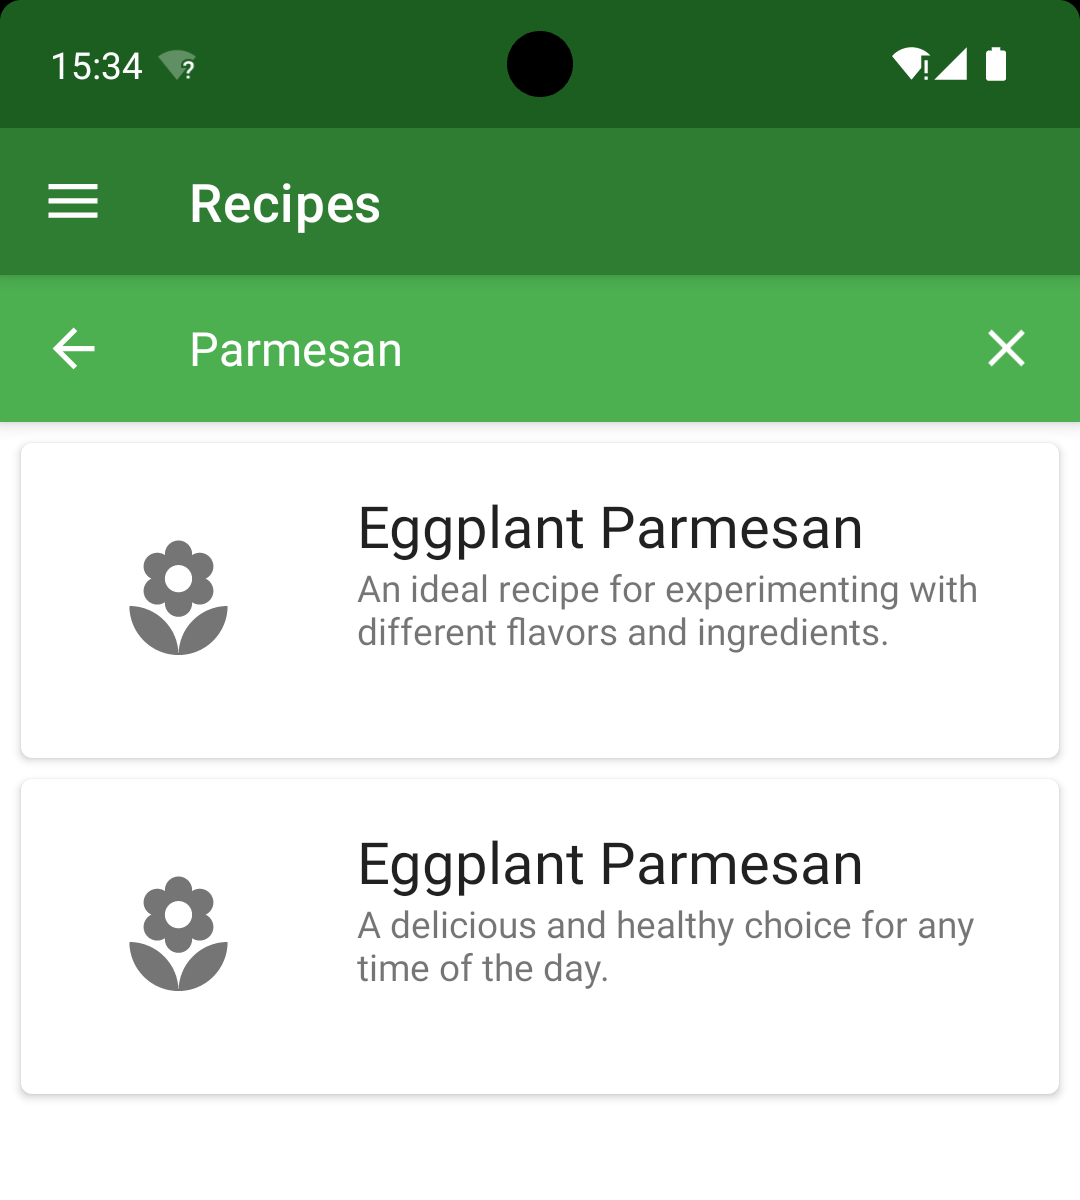
\includegraphics[width=0.485\linewidth]{figures/cases/android_recipe_search.png}}
    \hfill
    \fbox{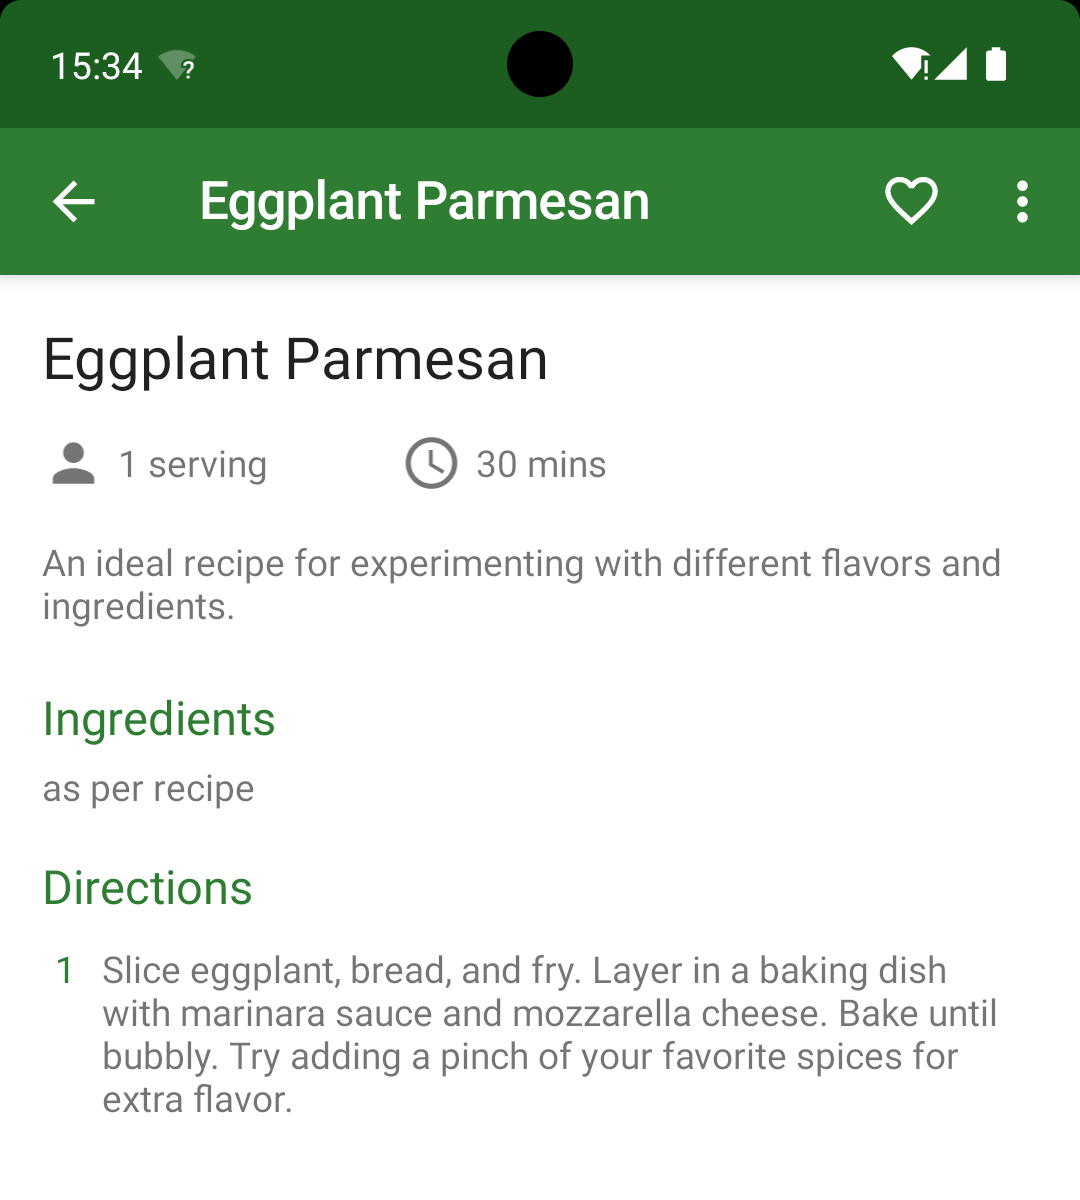
\includegraphics[width=0.485\linewidth]{figures/cases/android_recipe_detail.png}}

    \vspace{0.3em}

    {\footnotesize
    Screen 1: searched for \texttt{Parmesan}
    \hfill
    Screen 2: opened recipe details}
  \end{minipage}
  \hfill
  \begin{minipage}[t]{0.44\linewidth}
    \vspace{0pt}
    \vspace{-0.6em}

    % \footnotesize
    % \setlength{\abovecaptionskip}{2pt}

    \caption{
One case from \androidworld
(\href{https://github.com/google-research/android_world/blob/main/android_world/task_evals/single/recipe.py\#L133-L180}{source}).
The task asks the agent to delete recipes whose directions contain
\texttt{Parmesan}. The retained screens show the key trace: the agent
\textit{(i)} searches for \texttt{Parmesan}, \textit{(ii)} opens an
\texttt{Eggplant Parmesan} recipe, and \textit{(iii)} deletes nothing. The run
is nevertheless reported as successful because the released target construction
leaves the evaluator with an empty target set, while recipes treated as
non-targets mention \texttt{Parmesan}. This creates a false success label: the
benchmark output says the deletion succeeded.
    }

    \label{fig:recipe-motivation}
  \end{minipage}
\end{figure}

\begin{figure}[t]
  \centering
  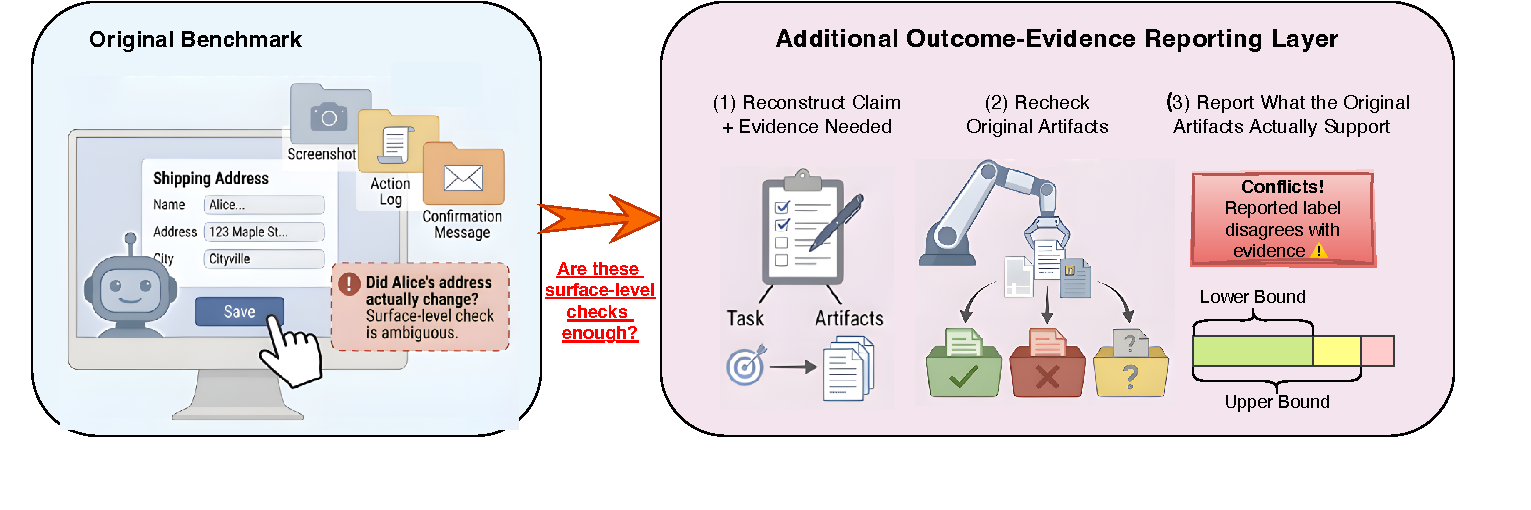
\includegraphics[width=\linewidth]{figures/diagram.pdf}
  \caption{Overview of the outcome-evidence gap and our reporting layer. A
  benchmark may report success from surface artifacts even when those artifacts
  do not verify the intended state change. Our layer leaves the benchmark run
  unchanged, then states the claim and needed evidence, rechecks the benchmark's
  saved artifacts, and reports what the original artifacts actually support:
  evidence labels, label conflicts, and evidence-supported bounds.}
  \label{fig:overview}
\end{figure}

We address this gap with an outcome-evidence reporting layer. The layer is
additive: it leaves benchmark tasks, agents, environments, and native
evaluators unchanged. For each case, it writes a short list of evidence needed
before scoring, specifying which stored artifacts would decide the
benchmark's own success claim. Each completed record is then labeled
\evidencePass, \evidenceFail, or \unknownLabel. Using \(P,F,U\) for the three
counts, the report keeps Unknown records visible rather than forcing them into
success, failure, or exclusion.

When a record is Unknown, none of the usual shortcuts is neutral. Counting it
as a success overstates what the evidence supports. Counting it as a failure
can punish missing instrumentation rather than agent behavior. Dropping it
changes which records are evaluated and can create agent-dependent
post-selection, because some agents leave more decisive traces than others. We
therefore keep Unknown records in the same set of completed records and
report the range of all-record performance still compatible with the stored
evidence. The
counted-only score is still useful, but only as a diagnostic conditional on
decidability, not as a headline all-record estimate.

We evaluate this reporting layer on four public interactive-agent benchmarks.
\agentdojo and \tauthree provide evidence-sensitive settings where plausible
traces can outrun stored evidence. \appworld and \webarena use strong
state-based or verified evaluators and serve as calibration controls. The study
is designed to be falsifiable: large Unknown shares on the controls would
indicate over-conservative evidence requirements, while narrow control bounds and
wider evidence-sensitive bounds would show that the layer distinguishes weak
stored evidence from strong native verification.

The paper makes four contributions: \textit{(i)} we formalize the
outcome-evidence gap in interactive-agent benchmarks, where a binary success
claim may be reported even when stored artifacts are insufficient to decide
that claim; \textit{(ii)} we introduce case checklists tied to
each benchmark's own success claim, plus a three-state counting rule that
separates \evidencePass, \evidenceFail, and \unknownLabel records
without changing benchmark tasks, agents, environments, or native evaluators;
\textit{(iii)} we derive evidence-supported performance bounds over the fixed
set of completed records, making the counted-only score a diagnostic over
decidable records rather than a headline all-record estimate; and
\textit{(iv)} we apply the method to four public benchmarks, showing that
evidence uncertainty is concentrated in evidence-sensitive domains while
remaining narrow on strong state-based evaluator controls, and release the
case checklists, reason labels, audit checks, robust-ranking summaries, and
scoring script needed to reproduce the reports.

\section{Related Work and Preliminaries}
\label{sec:related-prelim}

\paragraph{Interactive-agent evaluation and outcome checks.}
Interactive-agent benchmarks evaluate agents that navigate interfaces, call
tools, and alter environment state. Web-agent benchmarks include WebShop
\citep{yao2022webshop}, Mind2Web \citep{deng2023mind2web}, VisualWebArena
\citep{koh2024visualwebarena}, WebArena \citep{zhou2023webarena}, and
BrowserGym \citep{lesellierdechezelles2024browsergym}. Tool-use and
stateful-interaction benchmarks include ToolBench-style tool-use benchmarks
\citep{toolbench2024}, \(\tau\)-bench \citep{yao2024tau}, \tauthree
\citep{barres2026tau3bench}, and ToolSandbox \citep{lu2025toolsandbox}. Broader
agent environments include \agentdojo \citep{agentdojo}, \androidworld
\citep{rawles2025androidworlddynamicbenchmarkingenvironment}, \workarena
\citep{workarena2024}, \osworld \citep{osworld2024}, and long-horizon
workplace settings such as TheAgentCompany \citep{xu2024theagentcompany}.
These benchmarks make interactive evaluation realistic, but realism alone does
not guarantee that a stored trace decides the outcome claim being reported.

\paragraph{Verified evaluators and benchmark validity.}
A recent line of work strengthens outcome checks through state-based or
verified evaluation, including the verified \webarena release
\citep{elhattami2025webarena}, \appworld database-state unit tests
\citep{appworld2024}, and SWE-bench Verified \citep{swebenchverified2024}.
Benchmark-validity work, including the Agentic Benchmark Checklist, argues that
construct validity, outcome validity, and reporting assumptions should be made
explicit \citep{kang2025agenticbenchmarks}. Our contribution is complementary:
rather than proposing a new environment, a stronger domain evaluator, or an
audit checklist, we add a cross-benchmark reporting layer that asks what the
stored artifacts of completed runs can support under each benchmark's own
claim. LLM-as-judge and trajectory-evaluation work
\citep{zheng2023judging, shi2024judgingjudges, lu2025agentrewardbench},
benchmark refresh or contamination studies
\citep{kiela2021dynabench, guan2025benchmark, yang2023rethinkingcontamination},
and empirical audits of benchmark solutions \citep{wang2025solved,
openai2026swebenchverified} are useful diagnostics, but they do not replace
evidence that a native outcome claim is decidable from stored artifacts.
Dataset and model reporting work similarly argues that evaluation artifacts
should make their assumptions visible \citep{gebru2021datasheets,
mitchell2019modelcards, ma2025sphere, pineau2021improvingreproducibility};
our unit is a completed interactive-agent record and the artifacts retained to
verify its outcome claim.

\paragraph{Claims, records, traces, and evidence.}
A \emph{case} specifies a task, the initial environment, the benchmark claim
being tested, and the evidence required to decide that claim. A benchmark claim
is the binary outcome statement the benchmark reports for a completed run, such
as whether a target record was updated, a message was sent, or a constraint was
violated. The \emph{native evaluator} is the benchmark's released mechanism for
turning its available artifacts into a success or failure label.

We use \emph{case unit} only for a small bookkeeping issue: in most domains,
one task instance is one case unit, while in paired-arm settings such as
\agentdojo, two runnable arms form one case unit even though they are executed
separately. Decisions live at the level of \emph{records}. A record is one
agent's result on one case unit. The distinction matters because the same case
unit can be countable for one agent, whose trace exposes decisive evidence, and
Unknown for another, whose trace does not.

An \emph{episode} is one concrete execution of one agent on one runnable arm of
a case. Episodes produce \emph{traces}: ordered records of actions,
observations, tool calls, browser events, messages, files, and post-run
artifacts. We use \emph{stored artifacts} for the full set of traces, logs,
state snapshots, receipts, verifier inputs, and post-run measurements retained
after execution. \emph{Evidence} is the subset of those artifacts that can
support the active benchmark claim. A trace can be plausible without being
decisive.

\paragraph{Staying tied to the benchmark claim.}
Because the method sits on top of existing benchmarks, the requirements must
not silently make the task harder. For each case unit, we write down: (i) the
benchmark's own binary claim; (ii) the official source of that claim, such as
the task text, evaluator code, policy, or schema; (iii) the artifacts needed to
decide success or failure; (iv) the rule for assigning Unknown; and
(v) whether any requirement goes beyond the benchmark's own claim.

The requirements must be minimal with respect to the benchmark's own semantics.
For example, if a task says only ``update the address'' and the native
evaluator only checks the target record's address, then the requirements ask
for target-record identity and post-state evidence. A
no-collateral-change requirement is included only if the benchmark's own task,
policy, evaluator, or reported claim requires it. Otherwise it is labeled as a
stronger measurement claim and reported separately.

When sources differ, the requirements follow a fixed source hierarchy:
official evaluator semantics first; official task text and policy second; and
schema constraints needed to interpret evaluator-visible state third. We do not
add requirements from annotator intuition alone. Any requirement not grounded in
one of these sources is labeled as a stronger measurement claim and excluded
from the main bounds tied to the benchmark's own claim.

\section{Method}
\label{sec:evidence-reporting}
\label{sec:evidence-counting}
\label{sec:method}

The method turns completed benchmark runs into an evidence-supported report. It
keeps the benchmark's native view, namely the released evaluator's pass/fail
label, and adds an evidence view that asks whether the stored artifacts are
sufficient to decide the same underlying outcome claim. The layer is post-run
with respect to agent execution, but fixed before evidence scoring: it does not
change the task, prompt, agent, environment, native evaluator, or native score.

\paragraph{What Unknown means.}

Unknown is not a third kind of agent behavior. A record receives the Unknown
label when the available artifacts do not decide whether the benchmark's own
success claim is true. A clicked \texttt{Save} button, a final confirmation
message, or a passed proxy check may be insufficient if the retained state does
not show that the intended record changed. Conversely, timeouts, invalid
actions, tool misuse, and aborts after task start are failures when the native
benchmark would fail them; they are not moved into Unknown. In an ideal
state-based benchmark with explicit claims, aligned evaluators, complete
retained state, and unique entity mappings, Unknown records should be rare or
absent. Their presence measures an evidence gap in the benchmark report, not
task difficulty or agent uncertainty.

\paragraph{Case checklist.}

For each case unit, we first make the outcome claim explicit. An LLM-assisted
drafter reads the user goal, task text, official policy when present, released
evaluator or oracle code, and relevant state schemas. It proposes a compact
case checklist: what the user is trying to achieve, what condition the
benchmark reports as success, which official code or oracle checks that
condition, which artifacts would decide it after execution, and when the record
should remain undecided. For every checklist field filled by the LLM-assisted
drafter, the checklist must include either a rationale or a source pointer
identifying the file and location from which the information was derived. Human
reviewers source-check each checklist against the hierarchy in
Section~\ref{sec:related-prelim}. The checklist is not a new task or answer
key; it states what stored evidence would be sufficient to verify the
benchmark's own claim. In addition, the LLM-assisted drafter may propose
conditions that would require a stronger measurement claim, together with a
brief rationale for why those conditions go beyond the benchmark's native
success criterion. Human reviewers then adjudicate whether each proposed
stronger measurement claim is reasonable and sufficiently supported. We report
results in two layers: the native-aligned result, which follows the benchmark's
original claim, and a separate stronger-measurement result, which applies the
additional reviewed conditions.

\paragraph{Evidence scoring.}

We then run the benchmark normally and retain the artifacts available for
review: traces, tool calls, evaluator inputs and outputs, final messages, and
saved database, browser, file, or API state. For each completed record, the
native view records the released evaluator's label. The evidence view applies
the locked case checklist to the stored artifacts and assigns one of
three labels: \evidencePass, if the artifacts support success under the
benchmark claim; \evidenceFail, if they support failure; and \unknownLabel, if
they do not decide the claim. For every judgment made or proposed by an
LLM-assisted scorer, the
record must include either a rationale or a source pointer identifying the file
and location from which the information was derived. When a checklist includes
reviewed stronger-measurement conditions, we report the evidence results in two
layers: a native-aligned result, which follows the benchmark's original claim,
and a separate stronger-measurement result, which applies the additional
reviewed conditions. Thus the evidence view is an additional report over the
same runs, not a replacement for the native benchmark score.

\paragraph{Counting rule.}
\label{sec:bounds}

The reporting rule uses only the three evidence-state counts. For agent \(a\)
in domain \(d\), let \(N_{a,d}\) be the number of completed records in the
evaluation set, and let \(P_{a,d}\), \(F_{a,d}\), and \(U_{a,d}\) be the counts
of \evidencePass, \evidenceFail, and \unknownLabel records, so
\(N_{a,d}=P_{a,d}+F_{a,d}+U_{a,d}\). The counted-only
score answers a conditional question: among records the stored artifacts
decide, what fraction are successes? The bound answers the all-record question:
over every completed record, what performance values are still compatible with
the stored evidence? Writing \(P,F,U,N\) for the counts in a given agent-domain
cell, we report
\[
\mathrm{CountedScore}_{r}(a,d)=\frac{P}{P+F},\quad
\mathrm{Perf}_{r}(a,d)\in\left[\frac{P}{N},\frac{P+U}{N}\right],\quad
\mathrm{Width}_{r}(a,d)=\frac{U}{N}.
\]
The lower endpoint counts only Evidence Pass records; the upper endpoint treats
every Unknown record as a possible success. The width is exactly the Unknown
share. When \(U=0\), the bound collapses to the all-record score.
When \(U>0\), a single point estimate must make an unobserved decision about
records the artifacts did not decide. These intervals are not confidence
intervals; they are partial-identification bounds describing what the stored
evidence can and cannot identify \citep{manski2003partial}. The counted-only
score remains useful as a diagnostic conditional on decidability, but the
headline object is the evidence-supported bound.

\paragraph{Comparisons and diagnostics.}
\label{sec:interval-meaning}
\label{sec:pairwise}

We keep three diagnostics separate from the headline bounds. First,
case-cluster bootstrap intervals describe sensitivity to the finite set of
sampled cases. Each replicate resamples case units within a domain and keeps
all agent records attached to the resampled case unit. These intervals
condition on the stored traces and fixed agent versions; they do not measure
uncertainty from repeated executions, API drift, tool nondeterminism, or
environment volatility.

Second, pairwise rankings are supported only when the bounds separate. For
agents \(i\) and \(j\) in domain \(d\), the bound-implied difference interval
is \(\Delta(i,j;d)=[\mathrm{LB}_{i,d}-\mathrm{UB}_{j,d},
\mathrm{UB}_{i,d}-\mathrm{LB}_{j,d}]\). We report \(i\succ j\) only if
\(\mathrm{LB}_{i,d}>\mathrm{UB}_{j,d}\), and \(j\succ i\) only if
\(\mathrm{LB}_{j,d}>\mathrm{UB}_{i,d}\). Otherwise the pair is not identified
and is marked ``?'' rather than a tie. For a separated ordering \(i\succ j\),
the dominance margin is \(M_{i>j}=\mathrm{LB}_{i,d}-\mathrm{UB}_{j,d}\). We add
an asterisk when the 2.5th percentile of the case-cluster bootstrap distribution
of \(M_{i>j}\) remains positive; it marks descriptive stability, not
significance.

Third, every \(U\) record receives one reason, so the bound width can be
audited. The reasons are: missing state query (needed backend or environment
state was not saved), unobservable side effect (the consequence of an action is
not exposed), ambiguous identity mapping (the acted-on record or recipient is
not unique), missing state-preservation evidence (the native claim requires
unrelated state to remain unchanged but no diff or snapshot is available),
paired-arm asymmetry (one arm of a paired case is decidable and the other is
not), evaluator-output ambiguity (the released evaluator emits a label but the
stored inputs do not determine it), and claim-scope mismatch (the trace
supports a related task but not the reported claim). Appendix~\ref{app:unresolve-taxonomy}
gives representative examples and the priority rule used when more than one
reason could apply.

\section{Experiments}
\label{sec:study-design}
\label{sec:experimental-setup}
\label{sec:experiments}

We evaluate whether the reporting layer changes what benchmark scores can
claim, not which model wins a leaderboard. The experiment fixes four public
interactive-agent benchmarks, three current frontier agents, and a 100-case
sample per benchmark. Each run is scored twice: once by the benchmark's native
evaluator and once by the evidence-supported reporting layer.

\subsection{Benchmarks}

The benchmark suite contains two strong-evaluator controls and two domains
where the native claim can depend on evidence that is not always stored. This
mix is important: a useful reporting layer should leave strong native
verification mostly narrow while exposing uncertainty when traces are
insufficient. Across domains, the evidence view uses the artifacts retained by
the normal benchmark run, including traces, tool calls, evaluator inputs and
outputs, final messages, and saved database, browser, file, or API state when
available.

\begin{table}[t]
\centering
\caption{Benchmark suite. Each benchmark contributes 100 case units and is run
with three agents. The suite pairs two evidence-sensitive domains with two
strong-evaluator controls.}
\label{tab:domains}
\small
\setlength{\tabcolsep}{6pt}
\renewcommand{\arraystretch}{1.12}
\begin{tabularx}{\linewidth}{@{}l l >{\raggedright\arraybackslash}X@{}}
\toprule
Benchmark & Study role & Native check \\
\midrule
\tauthree & Evidence-sensitive & Retail-state success signal. \\
\agentdojo & Evidence-sensitive & Paired utility/security labels. \\
\appworld & Control & Database-state unit tests. \\
\webarena & Control & Verified deterministic evaluator. \\
\bottomrule
\end{tabularx}
\end{table}

\subsection{Agents and workload}
\label{sec:agents}

We run three agents through OpenRouter: Agent A is OpenAI GPT-5.4, Agent B is
Claude Opus 4.7, and Agent C is DeepSeek V4 Pro. All three use temperature
\(0\), a 4096-token output budget, a 120-second timeout, and two retries. The
paper does not treat these models as an exhaustive comparison set. They are
fixed measurement probes used to test whether outcome-evidence uncertainty is a
property of benchmark evidence rather than an artifact of one agent family. The
release records concrete model identifiers, prompts, tool wrappers, run dates,
and API settings.

For each benchmark, the manifest selects 100 eligible case units using a
deterministic hash order after excluding smoke-test and malformed cases. Each
case unit is run once per agent, giving \(4\times100\times3=1200\) completed
record slots before infrastructure exclusions. \agentdojo executes two arms per
record, so the main experiment stores 1500 execution episodes in total: 600 for
\agentdojo and 300 for each of the other three benchmarks.

\subsection{Execution and evidence scoring}

Every agent run uses the benchmark's original task interface, tools,
environment, and released evaluator. Evidence collection is handled by
benchmark-specific adapters that save raw run records, artifact manifests,
native evaluator outputs, traces, logs, and available post-run state. The
adapters do not make final evidence-label decisions, so the native score remains
directly recoverable from the saved artifacts.

Before evidence scoring, an LLM-assisted drafter produces one case checklist
per case unit. Drafting uses OpenAI GPT-5.4 through OpenRouter with
temperature \(0\), high reasoning effort, a 12,000-token output budget, and a
180-second timeout. The drafter receives the user goal, task
text, official policy when present, evaluator code or description, relevant
database/API/browser/file/tool schemas, and the schema of artifacts saved after
the run. Each LLM-filled checklist field must carry either a rationale or a
source pointer to the file and location that supports it. Two researchers
cross-validate the checklists in two review rounds. They check whether each
checklist follows the source hierarchy in Section~\ref{sec:related-prelim};
unsupported items are manually edited or regenerated and reviewed
again. Once locked, the checklists cannot be changed based on agent outcomes.
If the drafter proposes stronger-measurement conditions, reviewers adjudicate
them separately and score them outside the native-aligned result.

Final evidence scoring applies the locked checklist to each saved evidence
directory using Codex CLI with GPT-5.4, xhigh reasoning effort, a read-only
sandbox, and at most two attempts. The scoring bundle stores the score file,
manifest, stdout/stderr logs, telemetry, event stream, and reasoning summary so
that each Evidence Pass, Evidence Fail, or Unknown judgment can be audited.

\paragraph{Denominator rule.}
Only infrastructure or pre-run failures are excluded from the evaluation set.
Examples include a sandbox that fails to boot before the task is
presented, a missing benchmark asset, or an external service outage that
prevents normal benchmark execution. Agent-caused invalid actions, tool misuse,
timeouts after task start, malformed final answers, or benchmark-facing aborts
are not excluded. They are counted as failures when the native benchmark would
fail the run, and they are also reported in the all-attempt audit in
Table~\ref{tab:denominator-audit}. This separation prevents evidence
filtering from raising scores by removing difficult or agent-induced failures.

\paragraph{Sample size and precision.}
The primary unit for uncertainty is the case unit, not the record. Each benchmark
has 100 case units crossed with three agents, and the three records attached to a
case unit can be correlated because the agents face the same task. We therefore
avoid formal precision claims based on 300 independent records per benchmark. A
record-level binomial calculation would be, at best, an independence lower bound
and is not used for inference. All resampling intervals are case-clustered and
condition on the stored traces.

\subsection{Audit checks}
\label{sec:audit}

We run two checks for inspectability. First, two researchers audit 100 records,
25 per benchmark. The sample is stratified within each benchmark to include
decidable records, Unknown records, and native/evidence disagreements when all
three buckets are present. Auditors see the task, trace, artifacts, and locked
checklist, but not agent identity, native label, evidence label, or Unknown
reason.

Second, we rerun a fixed reference agent, OpenAI GPT-5.4, on ten case units per
benchmark. This rerun subset checks whether evidence labels are stable under a
small repeated-execution probe. It is not used as an uncertainty interval for
agent performance.

\paragraph{Adoption note.}
Adopting the method on top of an existing benchmark requires writing one fixed
claim and one case checklist per case unit, then running the scoring script over stored
traces. The script returns Evidence Pass, Evidence Fail, and Unknown counts,
coverage, counted-only score, lower and upper bounds, bound width, and
Unknown-reason records.

\section{Evaluation}
\label{sec:main-results}
\label{sec:evaluation}

The evaluation is organized around the questions a reader of an agent
benchmark actually needs answered. What did the original benchmark report? How
much of that report is directly supported by stored artifacts? If support is
missing, how large is the uncertainty, where does it come from, and does it
change model comparisons? The tables below specify exactly what evidence a
final benchmark report should expose. We interpret the Unknown share as a
property of stored benchmark evidence, not as an agent error rate.

\subsection{Evaluation 1: Evidence support for reported scores}
\label{sec:countability}

The first result is the score report itself. Table~\ref{tab:main-results-A}
keeps the native benchmark score visible, then adds the evidence view:
Evidence Pass, Evidence Fail, and Unknown counts, coverage, the counted-only
score, and the lower and upper endpoints. This table should let a
reader tell the difference between two very different situations: a native
score that is backed by nearly complete stored evidence, and a native score
whose apparent precision comes from treating Unknown records as if they had
been decided. Unless otherwise marked, the main tables report the
native-aligned layer. Stronger-measurement results are reported separately in
Appendix~\ref{app:supplemental-results} so that the paper does not silently
turn a benchmark into a stricter benchmark.

\begin{table*}[t]
\centering
\caption{Main measurement report. Counts are over completed records after
excluding only infrastructure/pre-run failures. Native score is the released
benchmark score on the same completed records. Coverage is the share of records
that stored artifacts decide. Counted-only score is conditional on those
decidable records. Lower and Upper are the all-record evidence-supported
endpoints; Width is the Unknown share.}
\label{tab:main-results-A}
\footnotesize
\setlength{\tabcolsep}{3pt}
\renewcommand{\arraystretch}{1.12}
\resizebox{\textwidth}{!}{%
\begin{tabular}{@{}lrrrrrrrrrr@{}}
\toprule
Benchmark & Total & Native score & E-Pass & E-Fail & Unknown & Coverage & Counted-only score & Lower & Upper & Width \\
\midrule
\tauthree & \TAUTotal & \TAUNativeScore & \TAUSuccess & \TAUFail & \TAUUnresolve & \TAUCoverage & \TAUCountedScore & \TAULower & \TAUUpper & \TAUWidth \\
\appworld & \APPTotal & \APPNativeScore & \APPSuccess & \APPFail & \APPUnresolve & \APPCoverage & \APPCountedScore & \APPLower & \APPUpper & \APPWidth \\
\webarena & \WAVTotal & \WAVNativeScore & \WAVSuccess & \WAVFail & \WAVUnresolve & \WAVCoverage & \WAVCountedScore & \WAVLower & \WAVUpper & \WAVWidth \\
\agentdojo & \ADJTotal & \ADJNativeScore & \ADJSuccess & \ADJFail & \ADJUnresolve & \ADJCoverage & \ADJCountedScore & \ADJLower & \ADJUpper & \ADJWidth \\
\midrule
All benchmarks & \ALLTotal & \ALLNativeScore & \ALLSuccess & \ALLFail & \ALLUnresolve & \ALLCoverage & \ALLCountedScore & \ALLLower & \ALLUpper & \ALLWidth \\
\bottomrule
\end{tabular}%
}
\end{table*}

\begin{figure}[t]
\centering
\fbox{\begin{minipage}{0.92\linewidth}
\textbf{Placeholder: native score and evidence-supported endpoints.}
\vspace{0.35em}

Final figure: one row per benchmark and model. Plot the native score, the
counted-only diagnostic score, and the evidence-supported interval
\([\mathrm{Lower},\mathrm{Upper}]\). Sort rows by Width.
\end{minipage}}
\caption{Planned visual summary of Table~\ref{tab:main-results-A} at the
model-by-benchmark level. The figure should make the paper's main empirical
pattern visually falsifiable: strong state-based benchmarks should have narrow
intervals, while evidence-sensitive benchmarks may have wide intervals.}
\label{fig:evidence-bound-plot}
\end{figure}

\subsection{Evaluation 2: Counted-only scores are conditional on decidability}
\label{sec:conditional-score}

The counted-only score answers a narrow but useful question: among records
where stored artifacts decide the benchmark claim, how often is success
supported? Its denominator is therefore not the full evaluation set when
Unknown records exist. In the final analysis, a high counted-only score with
low coverage should be described as ``high success on the decidable subset,''
not as strong all-record performance. Case-resampling intervals for the same
quantities appear in Appendix~\ref{app:supplemental-results}.

The next diagnostic asks why records are Unknown. Table~\ref{tab:unresolve-main}
should not be read as a new score; it is a repair map for benchmark authors.
If most Unknown records come from missing state queries, the fix is better
post-run state capture. If they come from identity ambiguity, the fix is
unique identifiers or stricter task schemas. If they come from claim-scope
mismatch, the benchmark needs a clearer statement of what its score claims.

\begin{table}[t]
\centering
\caption{Main Unknown-evidence diagnostic. Width is the Unknown share
from Table~\ref{tab:main-results-A}. The top reason identifies the largest
source of missing evidence; the final column should be filled with the concrete
benchmark repair suggested by that reason.}
\label{tab:unresolve-main}
\footnotesize
\setlength{\tabcolsep}{3pt}
\renewcommand{\arraystretch}{1.14}
\begin{tabularx}{\linewidth}{@{}l c X X@{}}
\toprule
Benchmark & Width & Top Unknown reason & Benchmark repair suggested by the evidence gap \\
\midrule
\tauthree & \TAUWidth & \TAUTopUnresolve & \fillfromdata \\
\appworld & \APPWidth & \APPTopUnresolve & \fillfromdata \\
\webarena & \WAVWidth & \WAVTopUnresolve & \fillfromdata \\
\agentdojo & \ADJWidth & \ADJTopUnresolve & \fillfromdata \\
\bottomrule
\end{tabularx}
\end{table}

\subsection{Evaluation 3: Model rankings require separated bounds}
\label{sec:robust-rankings}

The third result asks whether leaderboard comparisons survive Unknown
records. Table~\ref{tab:main-results-C} reports a directional ordering only
when one model's lower endpoint exceeds another model's upper endpoint. A
question mark means the ordering is not identified from stored evidence; it is
not a tie. This is deliberately stricter than comparing native point scores,
because the point scores may differ only inside the Unknown part of the
evaluation set.

\begin{table*}[t]
\centering
\caption{Directional pairwise robust-ranking matrix. Three agents induce three
pairwise comparisons per benchmark. A cell \(A>B\) is reported only when
\(\mathrm{LB}_{A,d}>\mathrm{UB}_{B,d}\); \(?\) denotes bound overlap. An
asterisk marks unadjusted case-resampling stability, not statistical
significance. It is added only when the observed bounds are separated and the
lower 2.5th percentile of the case-cluster bootstrap dominance margin remains
positive.}
\label{tab:main-results-C}
\footnotesize
\setlength{\tabcolsep}{3pt}
\renewcommand{\arraystretch}{1.14}
\resizebox{\textwidth}{!}{%
\begin{tabular}{@{}lcccr@{}}
\toprule
Benchmark & GPT-5.4--Claude 4.7 & GPT-5.4--DeepSeek V4 Pro & Claude 4.7--DeepSeek V4 Pro & Non-identified pairs \\
\midrule
\tauthree & \TAUpairAB & \TAUpairAC & \TAUpairBC & \TAUUnidentifiedPairs \\
\appworld & \APPpairAB & \APPpairAC & \APPpairBC & \APPUnidentifiedPairs \\
\webarena & \WAVpairAB & \WAVpairAC & \WAVpairBC & \WAVUnidentifiedPairs \\
\agentdojo & \ADJpairAB & \ADJpairAC & \ADJpairBC & \ADJUnidentifiedPairs \\
\midrule
All benchmarks & \multicolumn{3}{c}{Unsupported native strict orderings: \ALLUnsupportedNative; native conflicts: \ALLNativeConflicts} & \ALLUnidentifiedPairs \\
\bottomrule
\end{tabular}%
}
\end{table*}

\subsection{Evaluation 4: Counting decisions are inspectable}
\label{sec:inspectable}

The fourth result checks that the labels are not just another opaque judge.
The blinded audit samples counted records, Unknown records, and
native/evidence disagreements. The rerun subset checks whether labels remain
stable on a small repeated-execution probe. Disagreements are useful: they
identify cases where the requirement text, artifact capture, or reason
taxonomy needs clarification.

\begin{table}[t]
\centering
\caption{Stratified audit and rerun checks. Audit strata report counted
records, Unknown records, and native/evidence disagreements. Agreement and
\(\kappa\) values are descriptive for this stress sample, not unweighted
population estimates. Taxonomy \(\kappa\) uses \{R1--R7\} on items both
auditors marked Unknown. Rerun agreement checks label stability only.}
\label{tab:audit-rerun}
\footnotesize
\setlength{\tabcolsep}{3pt}
\renewcommand{\arraystretch}{1.14}
\begin{tabularx}{\linewidth}{@{}l r l r r r X@{}}
\toprule
Benchmark & Audit items & Audit strata & Audit agreement & Countability \(\kappa\) & Taxonomy \(\kappa\) & Rerun agreement / dominant disagreement \\
\midrule
\tauthree & 25 & \TAUAuditStrata & \TAUAuditAgreement & \TAUCountabilityKappa & \TAUTaxonomyKappa & \TAURerunAgreement; \TAURerunPattern \\
\appworld & 25 & \APPAuditStrata & \APPAuditAgreement & \APPCountabilityKappa & \APPTaxonomyKappa & \APPRerunAgreement; \APPRerunPattern \\
\webarena & 25 & \WAVAuditStrata & \WAVAuditAgreement & \WAVCountabilityKappa & \WAVTaxonomyKappa & \WAVRerunAgreement; \WAVRerunPattern \\
\agentdojo & 25 & \ADJAuditStrata & \ADJAuditAgreement & \ADJCountabilityKappa & \ADJTaxonomyKappa & \ADJRerunAgreement; \ADJRerunPattern \\
\midrule
All benchmarks & 100 & \ALLAuditStrata & \ALLAuditAgreement & \ALLCountabilityKappa & \ALLTaxonomyKappa & \ALLRerunAgreement; \ALLRerunPattern \\
\bottomrule
\end{tabularx}
\end{table}

\section{Discussion}
\label{sec:discussion}

The central empirical interpretation should be filled from
Table~\ref{tab:main-results-A} and Figure~\ref{fig:evidence-bound-plot}. In the
final version, this paragraph should state which benchmark has the largest
evidence gap, whether the strong-evaluator controls have narrow bounds, and
whether native scores fall inside the evidence-supported endpoints:
\fillfromdata. This is the main falsification check for the paper. If strong
state-based controls have wide bounds, the case checklists are too conservative
or the stored artifacts are weaker than expected; if evidence-sensitive domains
have wide bounds while controls remain narrow, the method is detecting a real
outcome-evidence difference rather than mechanically lowering scores.

The method is deliberately narrower than a new evaluator. It does not change
tasks, prompts, environments, agents, or the native score. Its claim is that a
benchmark report should distinguish what the released evaluator counted from
what stored artifacts can support. The discussion of rankings should therefore
be filled from Table~\ref{tab:main-results-C}: \fillfromdata. A non-identified
ordering is not a tie; it means the stored evidence supports more than one
completion of the Unknown records.

The bounds are also not confidence intervals. They are induced by Unknown
evidence. Case-cluster bootstrap intervals answer a separate question about
finite-case resampling conditional on stored traces and fixed agent versions.
The audit and rerun checks should be summarized here once filled:
\fillfromdata. Their role is inspectability, not a repeated-execution
performance estimate.

The main limitations follow from the design. A vague benchmark claim cannot be
rescued by a cleaner report; the seven-category Unknown-reason taxonomy is
a study vocabulary rather than a universal ontology; three agents are
measurement probes rather than a definitive leaderboard; and stronger-measurement
conditions must remain separate from the native claim. The practical
implication is direct:
benchmark reports should include Evidence Pass, Evidence Fail, and Unknown
counts, coverage, counted-only score, lower and upper endpoints, width, and
reason labels.
A benchmark can make the bounds collapse by retaining the state needed to
verify its own claim. Unknown records are therefore not an unavoidable
feature of interactive-agent evaluation; they are a diagnostic signal about
what a benchmark report does and does not substantiate.

\section{Conclusion}

Interactive-agent benchmarks often report scores over executed tasks, but
execution is not the same as evidence-supported measurement. We introduced a
reporting layer tied to each benchmark's own claim: it classifies completed
records as Evidence Pass, Evidence Fail, or Unknown, then reports the
evidence-supported bounds implied by Unknown records. Across \agentdojo,
\appworld, \webarena, and \tauthree, the evaluation asks whether uncertainty is
visible where stored artifacts do not decide the benchmark claim and remains
narrow where native evaluators already provide strong state-based evidence.
Future benchmark reports should include Evidence Pass, Evidence Fail, Unknown,
and bounds, so that a score is read together with the evidence that can
actually support it.

\clearpage
\bibliographystyle{plainnat}
\bibliography{ref}

\clearpage
\appendix

\section{Denominator Audit}
\label{app:denominator-audit}

\begin{table*}[h]
\centering
\caption{Denominator audit. Only infrastructure or pre-run failures are
excluded before forming the completed evaluation set. Agent-caused aborts,
invalid actions, and timeouts after task start stay in the denominator as
native failures.}
\label{tab:denominator-audit}
\footnotesize
\setlength{\tabcolsep}{2.6pt}
\renewcommand{\arraystretch}{1.18}
\begin{tabularx}{\textwidth}{@{}
>{\raggedright\arraybackslash}p{0.16\textwidth}
>{\centering\arraybackslash}p{0.09\textwidth}
>{\centering\arraybackslash}p{0.12\textwidth}
>{\centering\arraybackslash}p{0.09\textwidth}
>{\centering\arraybackslash}p{0.12\textwidth}
>{\raggedright\arraybackslash}X
@{}}
\toprule
Domain & Attempted & \shortstack{Infra/pre-run\\excluded} & Completed & \shortstack{Agent-caused\\fail} & Notes \\
\midrule
\agentdojo & \ADJAttempted & \ADJInfraExcluded & \ADJTotal & \ADJAgentCausedFail & Paired benign/injected arms remain linked at the case-unit level. \\
\appworld & \APPAttempted & \APPInfraExcluded & \APPTotal & \APPAgentCausedFail & Native database-state failures remain in the evaluation set. \\
\webarena & \WAVAttempted & \WAVInfraExcluded & \WAVTotal & \WAVAgentCausedFail & Browser-task timeouts after start remain in the evaluation set. \\
\tauthree & \TAUAttempted & \TAUInfraExcluded & \TAUTotal & \TAUAgentCausedFail & Tool misuse and policy-path failures remain in the evaluation set. \\
\midrule
All domains & \ALLAttempted & \ALLInfraExcluded & \ALLTotal & \ALLAgentCausedFail & Exclusions are not allowed to depend on whether the agent likely succeeded. \\
\bottomrule
\end{tabularx}
\end{table*}

\FloatBarrier

\section{Case Checklists and Scoring Inputs}
\label{app:requirement-drafting-details}

Before scoring, we create one fixed case checklist per sampled case unit. The
checklist is drafted with an LLM and then reviewed by two researchers in two
cross-validation rounds. The draft records the user's goal, what the official
benchmark oracle or evaluator checks, what actions or state changes are needed
for completion, and which stored artifacts would let a scorer decide the
benchmark's own claim. Every LLM-filled field must include either a rationale
or a source pointer to the file and location from which the information was
derived. If a draft item is unsupported, ambiguous, or stronger than the native
claim, reviewers edit it or regenerate that item and review it again. Proposed
stronger-measurement conditions are adjudicated separately and never folded
into the native-aligned result without being marked. The checklist is locked
before agent identities, agent traces, native scores, or evidence labels are
shown to the scorer.

After each run, we collect the stored artifacts and score the record twice: the
native benchmark evaluator gives the official/native label, and our scorer uses
the locked checklist to assign Evidence Pass, Evidence Fail, or Unknown. Any
LLM-assisted scoring judgment must also carry a
rationale or source pointer. This separation is important: the paper reports
both what the original benchmark would have counted and what the stored
artifacts can support under the additional case checklist.

\begin{table}[h]
\centering
\caption{Fields in the locked case checklist. The checklist is a scoring aid,
not a new task.}
\label{tab:case-checklist-fields}
\footnotesize
\setlength{\tabcolsep}{3pt}
\renewcommand{\arraystretch}{1.14}
\begin{tabularx}{\linewidth}{@{}l X X@{}}
\toprule
Field & Purpose & Required support \\
\midrule
User goal & Restates the task in benchmark language, including the intended object or recipient when available. & Task file, policy text, or rationale when the goal is synthesized across sources. \\
Native success claim & States what the released benchmark score claims to measure for this case. & Evaluator/oracle pointer, task text pointer, or policy pointer. \\
Official oracle or evaluator & Points to the official unit test, verifier, reward function, policy rule, or evaluator output used by the benchmark. & File path and code location, or released evaluator documentation. \\
Completion requirements & Lists the minimal state changes or side effects needed for the native claim to be true. & Source pointer for each requirement; rationale only when derived from multiple cited sources. \\
Evidence needed & Lists stored artifacts that can verify the claim, such as state diffs, database rows, receipts, verifier inputs, or unique identifiers. & Artifact schema pointer or rationale connecting the artifact to the native claim. \\
Evidence-label rule & Gives the scorer a deterministic rule for assigning Evidence Pass, Evidence Fail, or Unknown from stored artifacts. & Source pointer or rationale for each branch of the rule. \\
Stronger-measurement conditions & Separates reviewed non-native checks from the native-aligned result. & Brief rationale explaining why the condition goes beyond the native success criterion, plus reviewer adjudication. \\
Review notes & Records reviewer edits, regeneration reason, and final approval in two cross-validation rounds. & Reviewer id, round id, and decision note. \\
\bottomrule
\end{tabularx}
\end{table}

\begin{table}[h]
\centering
\caption{Case-checklist drafting metadata. These values are filled from the
scored manifest and released with the review package.}
\label{tab:requirement-drafting-metadata}
\footnotesize
\setlength{\tabcolsep}{4pt}
\renewcommand{\arraystretch}{1.14}
\begin{tabularx}{\linewidth}{@{}l X@{}}
\toprule
Field & Value \\
\midrule
Drafter provider and model & OpenRouter; OpenAI GPT-5.4 \\
Temperature / reasoning effort & \(0\); high \\
Output budget / timeout & 12,000 tokens; 180 seconds \\
Prompt version & \ChecklistPromptVersion \\
Visible inputs & Task text; official policy, if any; evaluator code or evaluator description; database/API/browser/file/tool schema; trace schema; available post-run artifact types \\
Hidden inputs & Agent identity; agent trace; native score; outcome label; alternate-view verdicts \\
Human review rule & Two researchers cross-validate every checklist in two rounds before scoring. Unsupported requirements are edited or regenerated, then rechecked. Requirements that go beyond the benchmark claim are adjudicated separately and kept out of the native-aligned result. \\
Source hierarchy & Evaluator semantics first; task text and policy second; schema constraints needed to interpret evaluator-visible state third. \\
\bottomrule
\end{tabularx}
\end{table}

\FloatBarrier

\section{Unknown-Reason Taxonomy}
\label{app:unresolve-taxonomy}
\label{sec:taxonomy}

Each Unknown record receives one upstream blocking reason. The labels make
missing evidence actionable for benchmark authors; they are not a universal
ontology.

\begin{table}[h]
\centering
\caption{Unknown-reason labels. The upstream-priority rule assigns
the reason that, if resolved first, would unblock the other missing evidence.}
\label{tab:unresolve-taxonomy}
\footnotesize
\setlength{\tabcolsep}{3pt}
\renewcommand{\arraystretch}{1.18}
\begin{tabularx}{\linewidth}{@{}l X X@{}}
\toprule
Reason & What is missing & Representative example \\
\midrule
R1: Missing state query & The benchmark claim depends on a backend or environment state value that was never queried or stored. & A database task has no post-run read of the relevant table. \\
R2: Unobservable side effect & The action is performed, but delivery, send, payment, receipt, or another side effect is not exposed in any artifact. & A message appears to be sent, but the tool returns no receipt or message id. \\
R3: Ambiguous identity mapping & Multiple records or recipients match the claim and the trace does not identify which one was acted on. & Two customers share the same name and no unique id is logged. \\
R4: Missing state-preservation evidence & The native task or policy requires preserving unrelated state, but no snapshot or diff can check it. & A calendar edit requires preserving other events, but no post-run diff is captured. \\
R5: Paired-arm asymmetry & A paired case requires both arms to be decidable, but one arm is decidable and the other is not. & The benign arm is verifiable while the injected arm's security claim is not. \\
R6: Evaluator-output ambiguity & The released evaluator emits a label, but its stored inputs do not uniquely support that label under the benchmark claim. & A verifier accepts a string match without evidence that the structured target state was reached. \\
R7: Claim-scope mismatch & The trace supports a related task, but not the benchmark claim being reported. & The agent gives a helpful refund response, but the policy-relevant backend update required by the claim is absent. \\
\bottomrule
\end{tabularx}
\end{table}

\FloatBarrier

\section{Additional Evaluation Tables}
\label{app:supplemental-results}
\label{app:per-agent}

The main text keeps only the tables needed to follow the argument. This section
holds the longer tables that will be filled directly from the scored manifest.

\begin{table}[h]
\centering
\caption{Per-agent evidence-supported bounds by benchmark. Each cell reports
native score, counted-only score, lower endpoint, upper endpoint, and width.}
\label{tab:per-agent}
\footnotesize
\setlength{\tabcolsep}{4pt}
\renewcommand{\arraystretch}{1.14}
\begin{tabularx}{\linewidth}{@{}l X X X@{}}
\toprule
Benchmark & OpenAI GPT-5.4 & Claude 4.7 & DeepSeek V4 Pro \\
\midrule
\agentdojo & \fillfromdata & \fillfromdata & \fillfromdata \\
\appworld & \fillfromdata & \fillfromdata & \fillfromdata \\
\webarena & \fillfromdata & \fillfromdata & \fillfromdata \\
\tauthree & \fillfromdata & \fillfromdata & \fillfromdata \\
\bottomrule
\end{tabularx}
\end{table}

\begin{table*}[h]
\centering
\caption{Stronger-measurement results. These rows apply only reviewed
conditions beyond the benchmark's native success criterion and are reported
separately from Table~\ref{tab:main-results-A}.}
\label{tab:stronger-measurement-results}
\footnotesize
\setlength{\tabcolsep}{3pt}
\renewcommand{\arraystretch}{1.14}
\begin{tabularx}{\textwidth}{@{}l X r r r r r r r X@{}}
\toprule
Benchmark & Stronger condition family & E-Pass & E-Fail & Unknown & Coverage & Lower & Upper & Width & Difference from native-aligned result \\
\midrule
\IfFileExists{outputs/latex/stronger_measurement_rows.tex}{\input{outputs/latex/stronger_measurement_rows.tex}}{%
\agentdojo & \fillfromdata & \fillfromdata & \fillfromdata & \fillfromdata & \fillfromdata & \fillfromdata & \fillfromdata & \fillfromdata & \fillfromdata \\
\appworld & \fillfromdata & \fillfromdata & \fillfromdata & \fillfromdata & \fillfromdata & \fillfromdata & \fillfromdata & \fillfromdata & \fillfromdata \\
\webarena & \fillfromdata & \fillfromdata & \fillfromdata & \fillfromdata & \fillfromdata & \fillfromdata & \fillfromdata & \fillfromdata & \fillfromdata \\
\tauthree & \fillfromdata & \fillfromdata & \fillfromdata & \fillfromdata & \fillfromdata & \fillfromdata & \fillfromdata & \fillfromdata & \fillfromdata \\
}
\bottomrule
\end{tabularx}
\end{table*}

\begin{table*}[h]
\centering
\caption{Descriptive case-resampling intervals for evidence-supported
quantities. These intervals condition on stored traces and fixed agent versions;
they do not include repeated-execution randomness, API drift, tool
nondeterminism, or environment volatility.}
\label{tab:main-results-B}
\footnotesize
\setlength{\tabcolsep}{3pt}
\renewcommand{\arraystretch}{1.14}
\begin{tabularx}{\textwidth}{@{}l X X X X X@{}}
\toprule
Domain & Lower endpoint & Upper endpoint & Width & Counted-only score & Native score inside bounds \\
\midrule
\agentdojo & \ADJLowerCI & \ADJUpperCI & \ADJWidthCI & \ADJCountedScoreCI & \ADJNativeInside \\
\appworld & \APPLowerCI & \APPUpperCI & \APPWidthCI & \APPCountedScoreCI & \APPNativeInside \\
\webarena & \WAVLowerCI & \WAVUpperCI & \WAVWidthCI & \WAVCountedScoreCI & \WAVNativeInside \\
\tauthree & \TAULowerCI & \TAUUpperCI & \TAUWidthCI & \TAUCountedScoreCI & \TAUNativeInside \\
\midrule
All domains & \ALLLowerCI & \ALLUpperCI & \ALLWidthCI & \ALLCountedScoreCI & \ALLNativeInside \\
\bottomrule
\end{tabularx}
\end{table*}

\begin{table*}[h]
\centering
\caption{Full Unknown-reason distribution. The main text reports the top
reason per benchmark; this table exposes the complete reason histogram.}
\label{tab:unresolve-reason-histogram}
\footnotesize
\setlength{\tabcolsep}{3pt}
\renewcommand{\arraystretch}{1.14}
\begin{tabularx}{\textwidth}{@{}lrrrrrrrX@{}}
\toprule
Benchmark & R1 & R2 & R3 & R4 & R5 & R6 & R7 & Interpretation \\
\midrule
\IfFileExists{outputs/latex/unresolve_reason_rows.tex}{\input{outputs/latex/unresolve_reason_rows.tex}}{%
\agentdojo & \fillfromdata & \fillfromdata & \fillfromdata & \fillfromdata & \fillfromdata & \fillfromdata & \fillfromdata & \fillfromdata \\
\appworld & \fillfromdata & \fillfromdata & \fillfromdata & \fillfromdata & \fillfromdata & \fillfromdata & \fillfromdata & \fillfromdata \\
\webarena & \fillfromdata & \fillfromdata & \fillfromdata & \fillfromdata & \fillfromdata & \fillfromdata & \fillfromdata & \fillfromdata \\
\tauthree & \fillfromdata & \fillfromdata & \fillfromdata & \fillfromdata & \fillfromdata & \fillfromdata & \fillfromdata & \fillfromdata \\
}
\bottomrule
\end{tabularx}
\end{table*}

\begin{table*}[h]
\centering
\caption{Pairwise dominance margins for bound-separated comparisons. For a
reported ordering \(i>j\), the margin is
\(M_{i>j}=\mathrm{LB}_{i,d}-\mathrm{UB}_{j,d}\). The bootstrap interval is a
descriptive stability check, not a formal significance test.}
\label{tab:pairwise-margins}
\footnotesize
\setlength{\tabcolsep}{3pt}
\renewcommand{\arraystretch}{1.14}
\begin{tabularx}{\textwidth}{@{}l l l l X@{}}
\toprule
Domain & Pair & Bound decision & Margin and case-resampling interval & Interpretation \\
\midrule
\IfFileExists{outputs/latex/pairwise_margin_rows.tex}{%
\input{outputs/latex/pairwise_margin_rows.tex}%
}{%
\textsc{fill from scored manifest} & -- & -- & -- & Include every bound-separated pair and its case-cluster bootstrap dominance margin.\\
}
\bottomrule
\end{tabularx}
\end{table*}

\FloatBarrier

\section{Reproduction Setup}
\label{app:reproduction-setup}

The released package separates checklist drafting, benchmark execution, and
evidence scoring. Paths in the table are release-relative; hostnames, live API
keys, and machine-specific absolute paths are not part of the public artifact.

\begin{table*}[h]
\centering
\caption{End-to-end reproduction pipeline. The adapter stage preserves raw
benchmark evidence and native evaluator outputs; final Evidence Pass, Evidence
Fail, and Unknown labels are assigned only in the scoring stage.}
\label{tab:reproduction-pipeline}
\footnotesize
\setlength{\tabcolsep}{4pt}
\renewcommand{\arraystretch}{1.16}
\begin{tabularx}{\textwidth}{@{}p{0.18\textwidth} X@{}}
\toprule
Stage & Reproduction details \\
\midrule
Checklist draft & Entry point: \texttt{make draft}. Model/configuration: OpenRouter OpenAI GPT-5.4, temperature \(0\), high reasoning effort, 12,000-token output budget, 180-second timeout. Input: \texttt{case\_packet.md}. Outputs: \texttt{checklist.yaml}, API response, LLM-call log, and reasoning summary. \\
Validation and locking & Entry point: offline checklist validator and case-lock update script. Inputs: \texttt{case\_packet.md} and draft checklist. Outputs: validated checklist and case-lock record. \\
Evidence collection & Entry point: benchmark-specific adapter over the official benchmark runner. Configuration: agent settings from \texttt{configs/agents.yaml}; no final evidence verdict. Inputs: \texttt{job.json}, benchmark installation, official assets, and agent config. Outputs: raw run record, artifact manifest, raw artifacts, native evaluator output, stdout/stderr, and call logs. \\
Evidence scoring & Entry point: \texttt{make score}. Model/configuration: Codex CLI GPT-5.4, xhigh reasoning effort, read-only sandbox, at most two attempts. Inputs: locked checklist and saved evidence directory. Outputs: score JSON/YAML, score manifest, stdout/stderr logs, event stream, telemetry, and reasoning summary. \\
\bottomrule
\end{tabularx}
\end{table*}

\begin{table}[h]
\centering
\caption{Agent-call configuration for the main experiment.}
\label{tab:agent-call-config}
\footnotesize
\setlength{\tabcolsep}{4pt}
\renewcommand{\arraystretch}{1.12}
\begin{tabularx}{\linewidth}{@{}l l X r r r@{}}
\toprule
Agent & Provider & Model & Temp. & Output budget & Timeout / retry \\
\midrule
A & OpenRouter & OpenAI GPT-5.4 & 0 & 4096 & 120 s / 2 \\
B & OpenRouter & Claude Opus 4.7 & 0 & 4096 & 120 s / 2 \\
C & OpenRouter & DeepSeek V4 Pro & 0 & 4096 & 120 s / 2 \\
\bottomrule
\end{tabularx}
\end{table}

\begin{table}[h]
\centering
\caption{Machine roles used for raw evidence collection. Drafting and final
scoring can run on any authenticated CPU machine and require no GPU.}
\label{tab:machine-routing}
\footnotesize
\setlength{\tabcolsep}{4pt}
\renewcommand{\arraystretch}{1.12}
\begin{tabularx}{\linewidth}{@{}l l l c@{}}
\toprule
Benchmarks & Machine role & Configuration & Docker \\
\midrule
\agentdojo, \appworld, \tauthree & General adapter VPS & 8 CPU, 32 GB memory, no GPU & Yes \\
\webarena & WebArena adapter VPS & 4 CPU, 16 GB memory, no GPU & Yes \\
\bottomrule
\end{tabularx}
\end{table}

\FloatBarrier

\section{Release and Result Files}
\label{app:release}
\label{app:macro-requirements}

Public release should make denominators and bounds auditable without exposing
live credentials, real third-party keys, or side-effecting services.

\begin{itemize}\itemsep0.15em
\item \textbf{Released publicly.} Case ids, locked case checklists, native
claim, checklist rationales or source pointers, stronger-measurement flags and
rationales, native label, evidence label, reason code, bound contribution,
denominator audit, aggregate tables, plotting scripts, and audit instructions.
\item \textbf{Released under access control when needed.} Full traces that
contain prompt-injection content, synthetic personal data, or credential-shaped
strings after scrubbing and sandbox re-pinning.
\item \textbf{Not released.} Live credentials, real API keys, or artifacts that
would reproduce side effects against non-sandboxed services.
\item \textbf{Versioning.} Reported bounds are paired with a version tuple for
the scorer, manifest, checklist template, checklist-generation prompt, and
Unknown-reason taxonomy.
\end{itemize}

The final build should be produced from the scored manifest. The file
\texttt{outputs/latex/results\_macros.tex} should set
\verb|\resultdatatrue| and define the domain-level macros used in
Tables~\ref{tab:main-results-A}--\ref{tab:main-results-C}. Optional row files
can populate the longer appendix tables. Missing values should remain visibly
marked as \fillfromdata rather than replaced by guessed numbers.
\clearpage
\IfFileExists{checklist.tex}{\clearpage\input{checklist.tex}}{}

\end{document}
